%--------------------------------------------------------------------------------------------------------------------------------%
%\PassOptionsToPackage{refsection=refsegment}{biblatex}
\documentclass{article}
\usepackage[utf8]{inputenc}
\usepackage[english]{babel}
\usepackage{geometry}
 \geometry{
 a4paper,
 total={170mm,257mm},
 left=20mm,
 top=20mm,
 bottom = 30mm,
 }
 
\usepackage[
backend=bibtex,
refsegment=section
]{biblatex}

\addbibresource{references.bib}

\defbibheading{subbibheading}{
  \section*{References for Section \ref{refsegment:\therefsection\therefsegment}}
}

\DeclareBibliographyCategory{skipbibliography}
\DeclareCiteCommand{\myfootcite}[\mkbibfootnote]
  {\usebibmacro{prenote}}
  {\addtocategory{skipbibliography}{\thefield{entrykey}}%
   \usedriver
     {\DeclareNameAlias{sortname}{default}}
     {\thefield{entrytype}}}
  {\multicitedelim}
  {\usebibmacro{postnote}}

\usepackage{graphicx}
\usepackage{hyperref}
\usepackage{url}
\usepackage{color,soul}
\usepackage{physics}
\usepackage{amsthm}
\usepackage[section]{placeins}

\newtheorem{theorem}{Theorem}[section]
\newtheorem{lemma}[theorem]{Lemma}

\usepackage{pythonhighlight}
\usepackage{algorithm}
\usepackage[noend]{algpseudocode}

\usepackage{float}
\usepackage{graphicx}

%--------------------------------------------------------------------------------------------------------------------------------%
\title{Introduction to Optics}
\author{Bryan Turo\\ \href{mailto:bryanturo@gmail.com}{Bryanturo@gmail.com} }

\date{April 2021}
%--------------------------------------------------------------------------------------------------------------------------------%

\begin{document}
\maketitle

\tableofcontents

\newpage


%--------------------------------------------------------------------------------------------------------------------------------%
\section{Introduction}
First of all, welcome to the beautiful field of Optics and Photonics.
\\
\
\\
The purpose of this document is to introduce someone with little to no history of optics to concepts which I found most important during my time working with Dr. Hebin Li\footnote{This opportunity was the single most important thing I did in my undergraduate career, do not waste it and take advantage of it to the fullest.} at FIU.
\\
\ 
\\
This field deals with the study of light-matter interactions, optics is composed of classical, semi-classical and quantum theories of light and their interactions. Let's split this into a couple major categories:
\begin{figure}[!phtb]
    \centering
    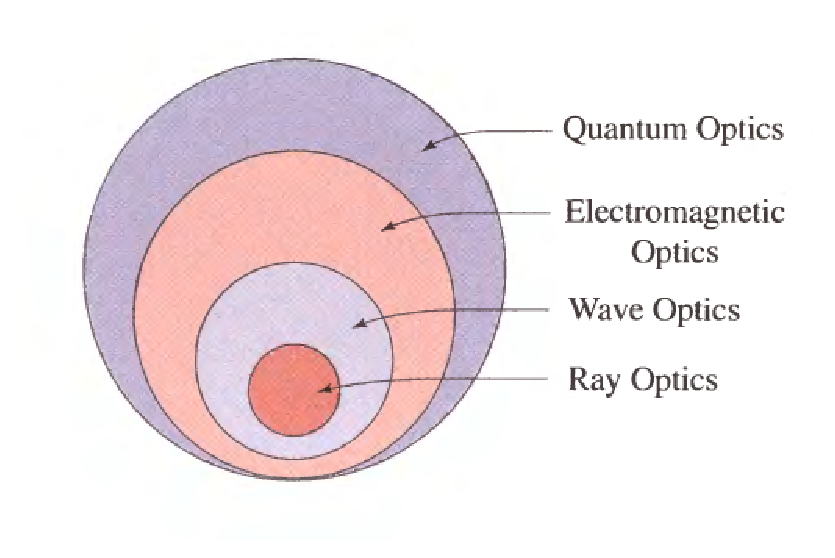
\includegraphics[width=0.75\linewidth]{img/categories.eps}
    \label{fig:categories}
\end{figure}

I will introduce the highlights of each section and reference different sources for learning the material.
\\
My recommendation of reading this document is to gather a surface level understanding of how different aspects of optics tie in together. This may lead to an easier time in understanding individual concepts at much greater depths.

I must repeat, this document is not a replacement for other references and should not be the only source of information at your disposal. Read the references attached and papers on the subject.
\newpage

%--------------------------------------------------------------------------------------------------------------------------------%
\section{Ray Optics}
\subsection{Thin Lens equation}
In introductory Physics 2 you will briefly learn about the (thin lens or spherical mirror) equation.
\begin{equation}
    \frac{1}{f} = \frac{1}{d_o} + \frac{1}{d_i}
\end{equation}
where, $f$ is focal distance, $d_0$ is object distance, and $d_i$ is image distance.
\\
\
\\
Use the idea of a magnifying glass to picture what the object and image is, the image is the magnified object you receive in your eye.
The \hl{magnification} of an image is given by
\begin{equation}
    m = -\frac{d_i}{d_o}
\end{equation}
Before I define focal length I want to introduce the concept of converging, diverging and parallel rays.

Imagine a \hl{point source} with an infinite density of rays, this is a diverging source.
\begin{figure}[!phtb]
    \centering
    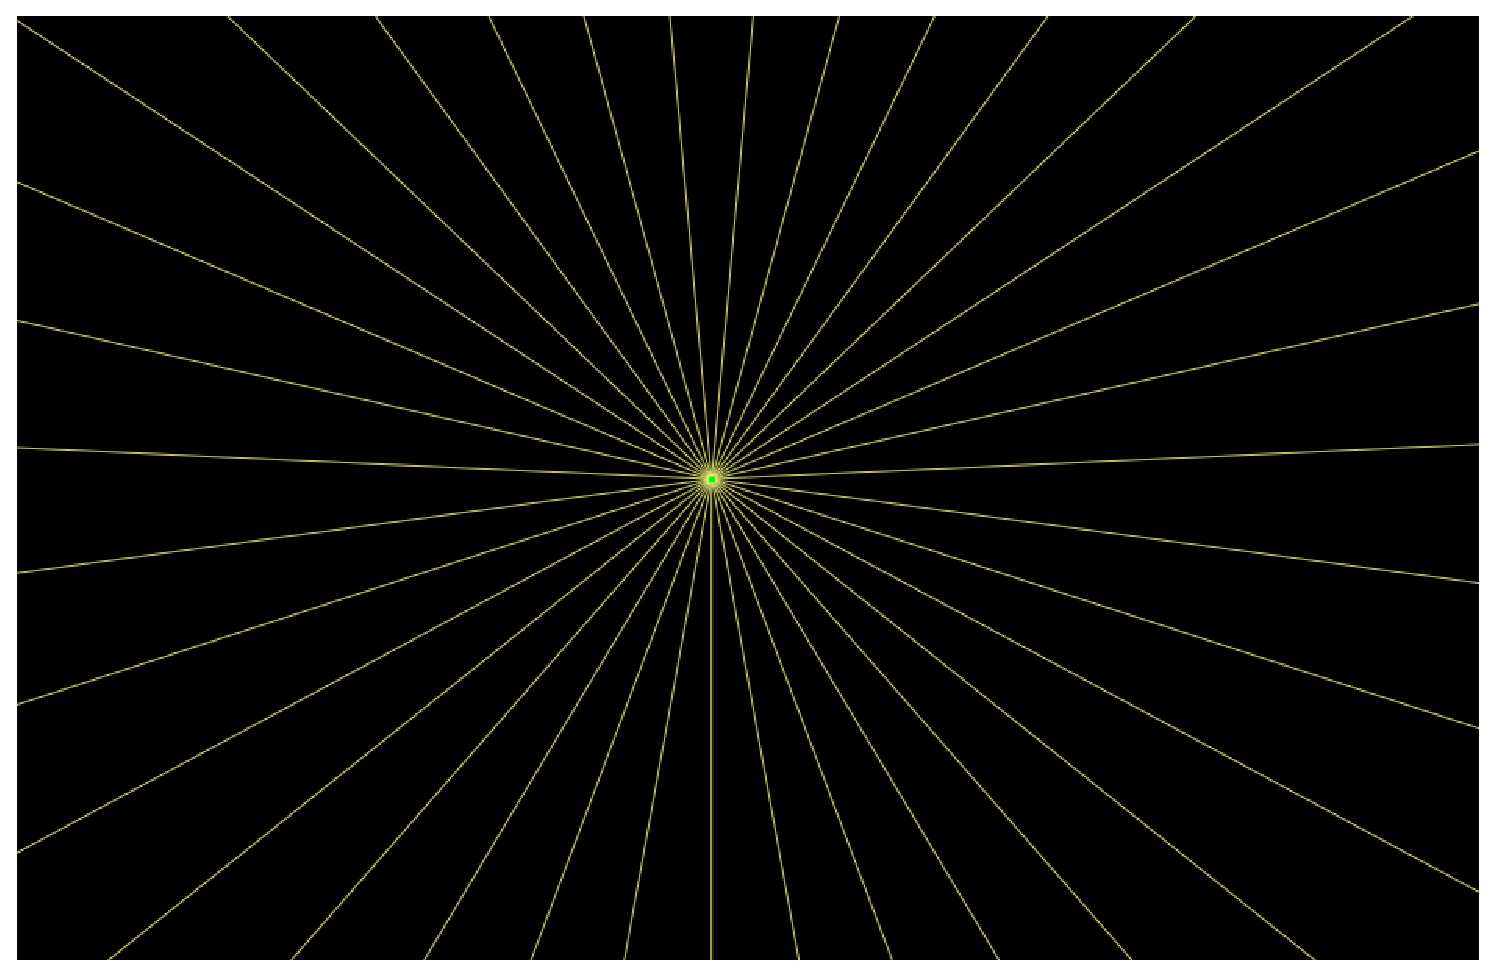
\includegraphics[width=0.6\linewidth]{img/PointSource.eps}
    \caption{A point source emitting rays of light}
    \label{fig:PointSource}
\end{figure}
\\
If we follow these rays to some distance $D$ to the right, we will begin to see that they become parallel with respect to each other.
As $D\rightarrow\infty$ we get perfectly parallel rays.
\\
\begin{figure}[!phtb]
    \centering
    \includegraphics[width=0.75\linewidth]{img/DAway.eps}
    \caption{At a distance D away you can begin to see how the rays become parallel}
    \label{fig:PointSource}
\end{figure}

\newpage

If we introduce a lens to these parallel rays you get a converging beam.
\begin{figure}[!phtb]
    \centering
    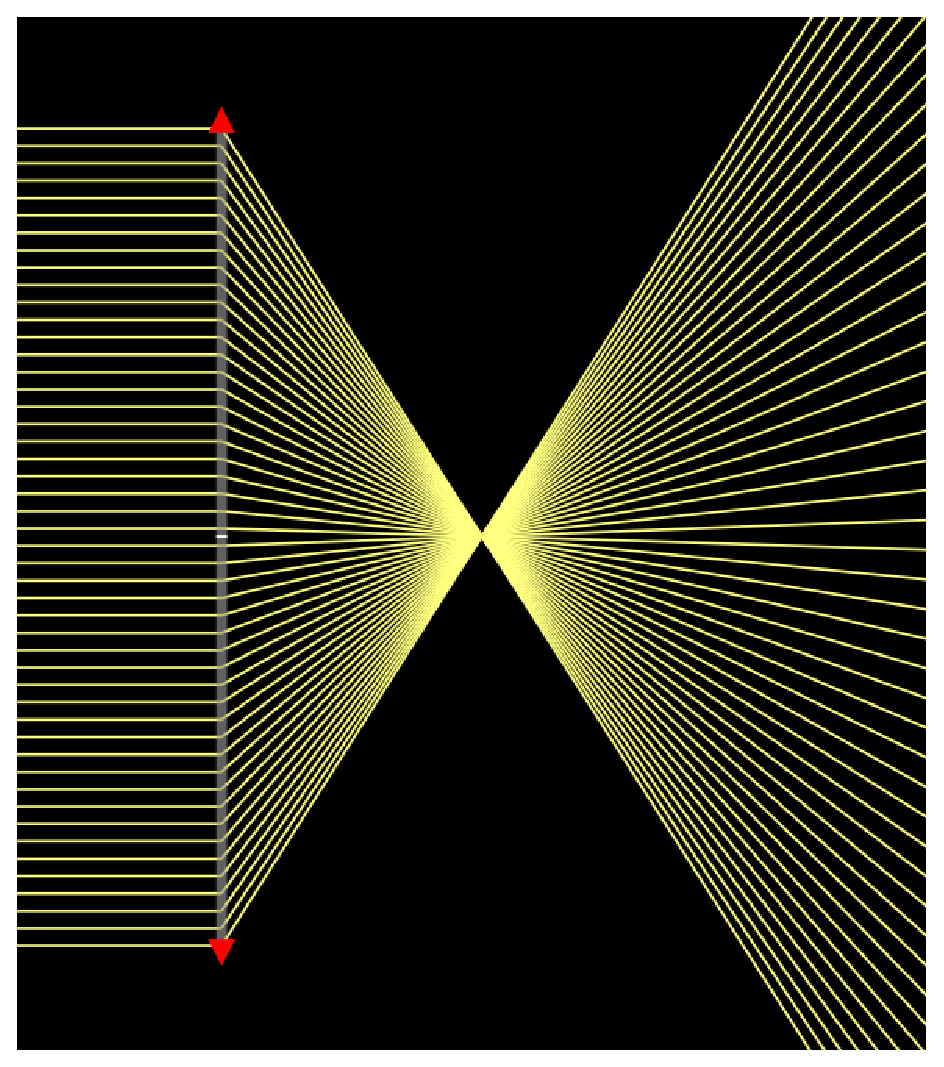
\includegraphics[width=0.5\linewidth]{img/Converging.eps}
    \caption{A lens converging a collimated beam}
    \label{fig:PointSource}
\end{figure}
\\
The focal length $f$ is given by the point at which the beam converges to.
\\
When rays are parallel to each other this is what is called \hl{\emph{collimated light.}}
\\
\\
Let's make sure we know how to use the thin lens equation.
If we place an object to the left of a lens at distance $d_o$ and the lens has a focal length $f$ then where does the image form if $d_o = f$
$$\frac{1}{f} = \frac{1}{d_o}+\frac{1}{d_i}= \frac{1}{f}+\frac{1}{d_i}$$
We get $$\frac{1}{d_i} = 0$$ which only occurs when $d_i \rightarrow \infty$
This means the image never forms and the beam of light is now collimated.

%--------------------------------------------------------------------------------------------------------------------------------%
\section{Wave Optics}
\subsection{The wave equation}
Ray optics is wave optics with the constraint of the wavelength to be infinitesimally short. Ray-optics theory is useful as long as the light waves interact with objects with dimensions much bigger than its wavelength.

Now, to cover the basics: light exhibits what we call particle-wave duality in which it acts as a wave propagating through space and as a particle when interacting with matter.

The solution to the wave equation that describes light is referred to as the wave-function. The wave equation is a partial differential equation with solution $u(\textbf{r},t)$ and is given by
\begin{equation}
    \grad^2u-\frac{1}{c^2}\frac{\partial^2u}{\partial t^2} = 0
    \label{eq:waveequation}
\end{equation}

If you have taken partial differential equations, you may know how to solve an equation like this, if not don't worry, just take the solution for granted.
One of the most important properties of these partial differential equations is the \emph{principle of superposition}:
\begin{lemma}
If $u_1(\textbf{r},t)$ and $u_2(\textbf{r},t)$ are both solutions to the wave-equation than their \hl{superposition} then $u(\textbf{r},t) = u_1(\textbf{r},t)+u_2(\textbf{r},t)$ is another solution.
\label{superposition_lemma}
\end{lemma}
Now, we can have different types of solutions for the wave equation, one of such solutions is that of a plane wave given by
\begin{equation}
    U(\textbf{r})=Ae^{-i(k_xx+k_yy+k_zz)}
\end{equation}
Which has a planar wave front.

Another is that of a spherical wave
\begin{equation}
    U(\textbf{r})=\frac{A}{r}e^{-ikr}
\end{equation}
Collimated light passing through a lens using wave theory can be represented by fig. \ref{fig:planarwave}
\begin{figure}[!phtb]
    \centering
    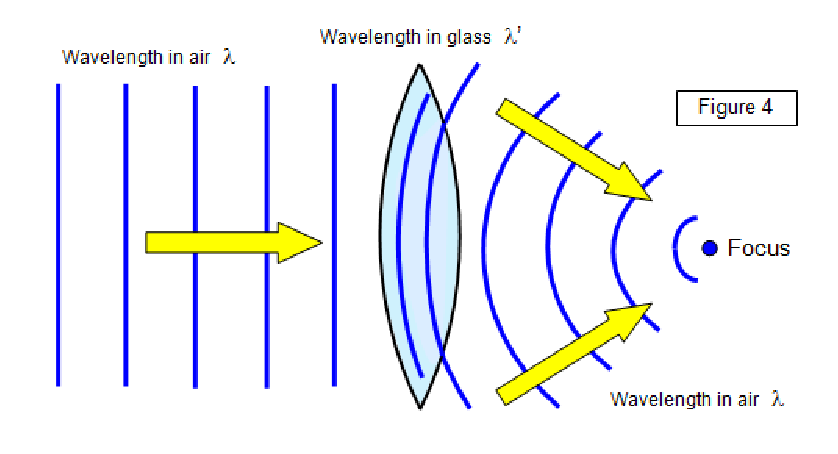
\includegraphics[width=0.5\linewidth]{img/planarwave.eps}
    \caption{Planar wave being transformed into a spherical wave by the lens.}
    \label{fig:planarwave}
    \nocite{schoolphysics}
\end{figure}
\\
So a good question now is, hey why does the lens cause the planar wave to convert into a spherical wave\footnote[1]{It actually isn't spherical, but rather paraboloidal, see references}?
\\
Light does not travel at the speed of light\footnote[2]{More on this when we get to EM Optics} (unless you're in a vacuum)

Light actually travels a little slower in different medium depending on the \hl{refractive index $n$} of the medium it passes through
\begin{equation}
    c = \frac{c_0}{n}
\end{equation}
Let's treat this refractive index property as intrinsic to the material and \textbf{wavelength dependent}.
\\
It is clear to see why the planar wave converts to a spherical wave now.



\subsection{Interference}
%TODO
If you have done the double slit experiment then you have dealt with interference effects before.

The premise is simple: if you have two waves $U_1(\textbf{r},t)$ and $U_2(\textbf{r},t)$ and they are superimposed spatially, then you will create a resultant wave.
\begin{equation}
    U(\textbf{r},t) = U_1(\textbf{r},t)+U_2(\textbf{r},t)
\end{equation}
When speaking of waves of light, it is useful to talk about the \hl{intensity of light}. This intensity I is related to the wave by
\begin{equation}
    I = \abs{U}^2
\end{equation}
In the case of interference,
\begin{equation}
    I = \abs{U}^2 = \abs{U_1+U_2}^2 = I_1 + I_2 + 2\sqrt{I_1 I_2}cos(\delta)
\end{equation}
Where $\delta$ is the \hl{phase difference} of the waves, $\delta = \delta_2-\delta_1$

This interference effect can be manipulated in many ways, such as in interferometers
\subsection{Diffraction Gratings}
Exploiting index of refraction and interference we get to the diffraction grating. A diffraction grating allows you to split an incoming wave into several waves called "orders". When shining polychromatic light (Light containing several wavelengths) onto a diffraction grating, the light is spread out by color since each wavelength has a different index of refraction.
\begin{figure}[!phbt]
    \centering
    \includegraphics[width=0.5\linewidth]{img/polychromatic.eps}
    \caption{Polychromatic light hitting a diffraction grating and splitting into different orders}
    \label{fig:polychromatic}
    \nocite{horiba}
\end{figure}
%--------------------------------------------------------------------------------------------------------------------------------%


\section{Electromagnetic Optics}
\subsection{Maxwell's Equations}
We have talked about the wave properties of light however, what exactly is propagating?
Light is an \hl{electro-magnetic wave} that satisfies Maxwell's Equations (Differential form).
\begin{equation}
    \begin{aligned}
        \nabla \cdot \mathbf{E} &= \frac {\rho} {\varepsilon_0} \\
        \nabla \cdot \mathbf{B} &= 0 \\
        \nabla \times \mathbf{E} &= -\frac{\partial \mathbf{B}} {\partial t} \\
        \nabla \times \mathbf{B} &= \mu_0 \mathbf{J} + \mu_0 \varepsilon_0 \frac{\partial \mathbf{E}} {\partial t} \\
    \end{aligned}
\end{equation}
Since the electric field (E-Field) and the magnetic field (M-Field) are dependent on each other, the solution to Maxwell's equations is a self-propagating planar wave with perpendicular E and M fields.
\begin{equation}
    \textbf{E} = \textbf{E}_0e^{i(kz - \omega t)}
\end{equation}
\begin{equation}
    \textbf{B} = \textbf{B}_0e^{i(kz - \omega t)}
\end{equation}
With $k = \frac{2\pi v}{c} = \frac{\omega}{c}$ which arises from the solution.

It looks like this,
\begin{figure}[!phtb]
    \centering
    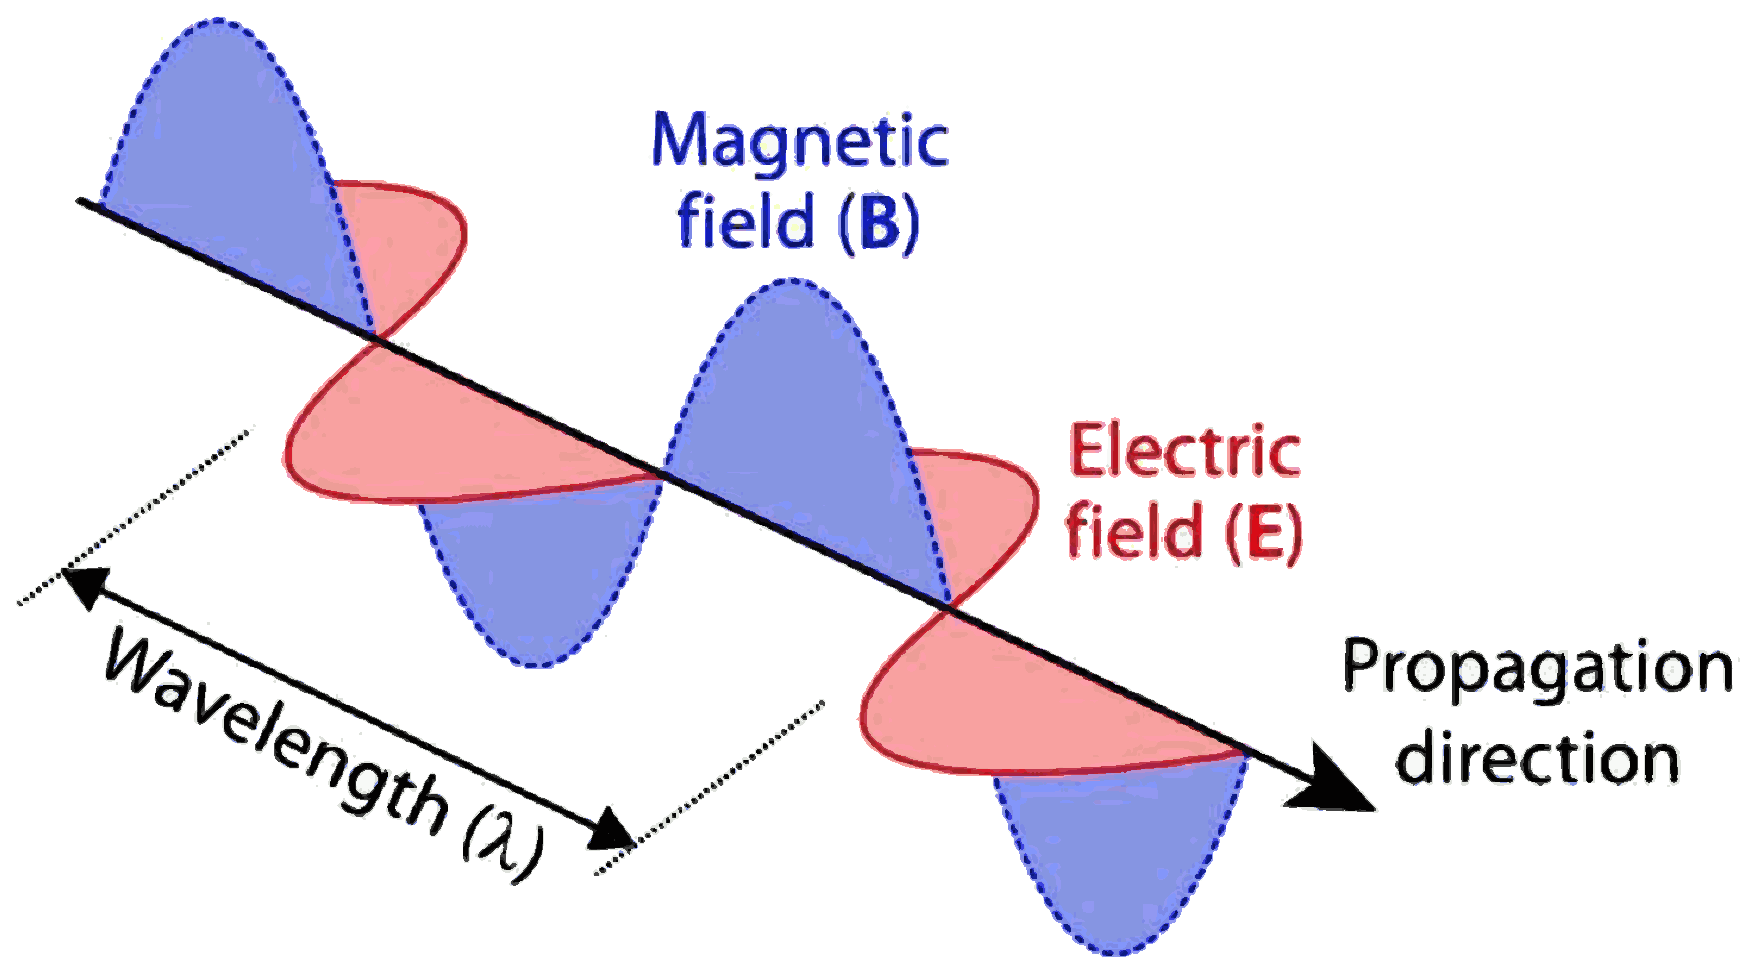
\includegraphics[width=0.6\linewidth]{img/EM_Wave.eps}
    \caption{Perpendicular E and M fields oscillating}
    \label{fig:EM_Wave}
\end{figure}

Defining the intensity of light to be
\begin{equation}
    I \propto \abs{\textbf{E}}^2
    \label{Intensity}
\end{equation}

We saw in the previous chapter that one solution to the wave equation is that of spherical waves, well although it is a useful concept mathematically: in reality there does not exist spherical waves as this solution is not allowed by Maxwell's equations. Let us think of spherical waves as the careful superposition of planar waves\footnote{More on this in Fourier Optics}

This is a nice depiction of an EM-wave however, one must note that EM fields fill all of 3-D space, the depiction in figure \ref{fig:EM_Wave} is useful for thinking of planar waves because the electric field oscillates in a single plane. As with everything, this is merely a useful concept to explain reality.

%--------------------------------------------------------------------------------------------------------------------------------%

\subsection{Polarization}
This is a very important section and should be understood very well.

In the last section, the electric field oscillating in a single plane was mentioned. This is actually quite an important concept and shall be the topic of discussion for explaining Polarization.


The sun releases approximately $10^{45}$ photons per second, that's a lot of photons. Let's consider fig. \ref{fig:EM_Wave}, here let's focus on the electric field of the EM-wave. Since the sun releases photons at random, each of the photons released by the sun have their electric field oscillating in a random plane, the superposition of the photons released by the sun give what is called \hl{Unpolarized light}.

Some materials only allow light to pass through if their electric field oscillates in a particular plane; these materials are called \hl{polarizers}.
Linearly polarized light that has electric fields propagating only in one plane.
\begin{figure}[!phbt]
    \centering
    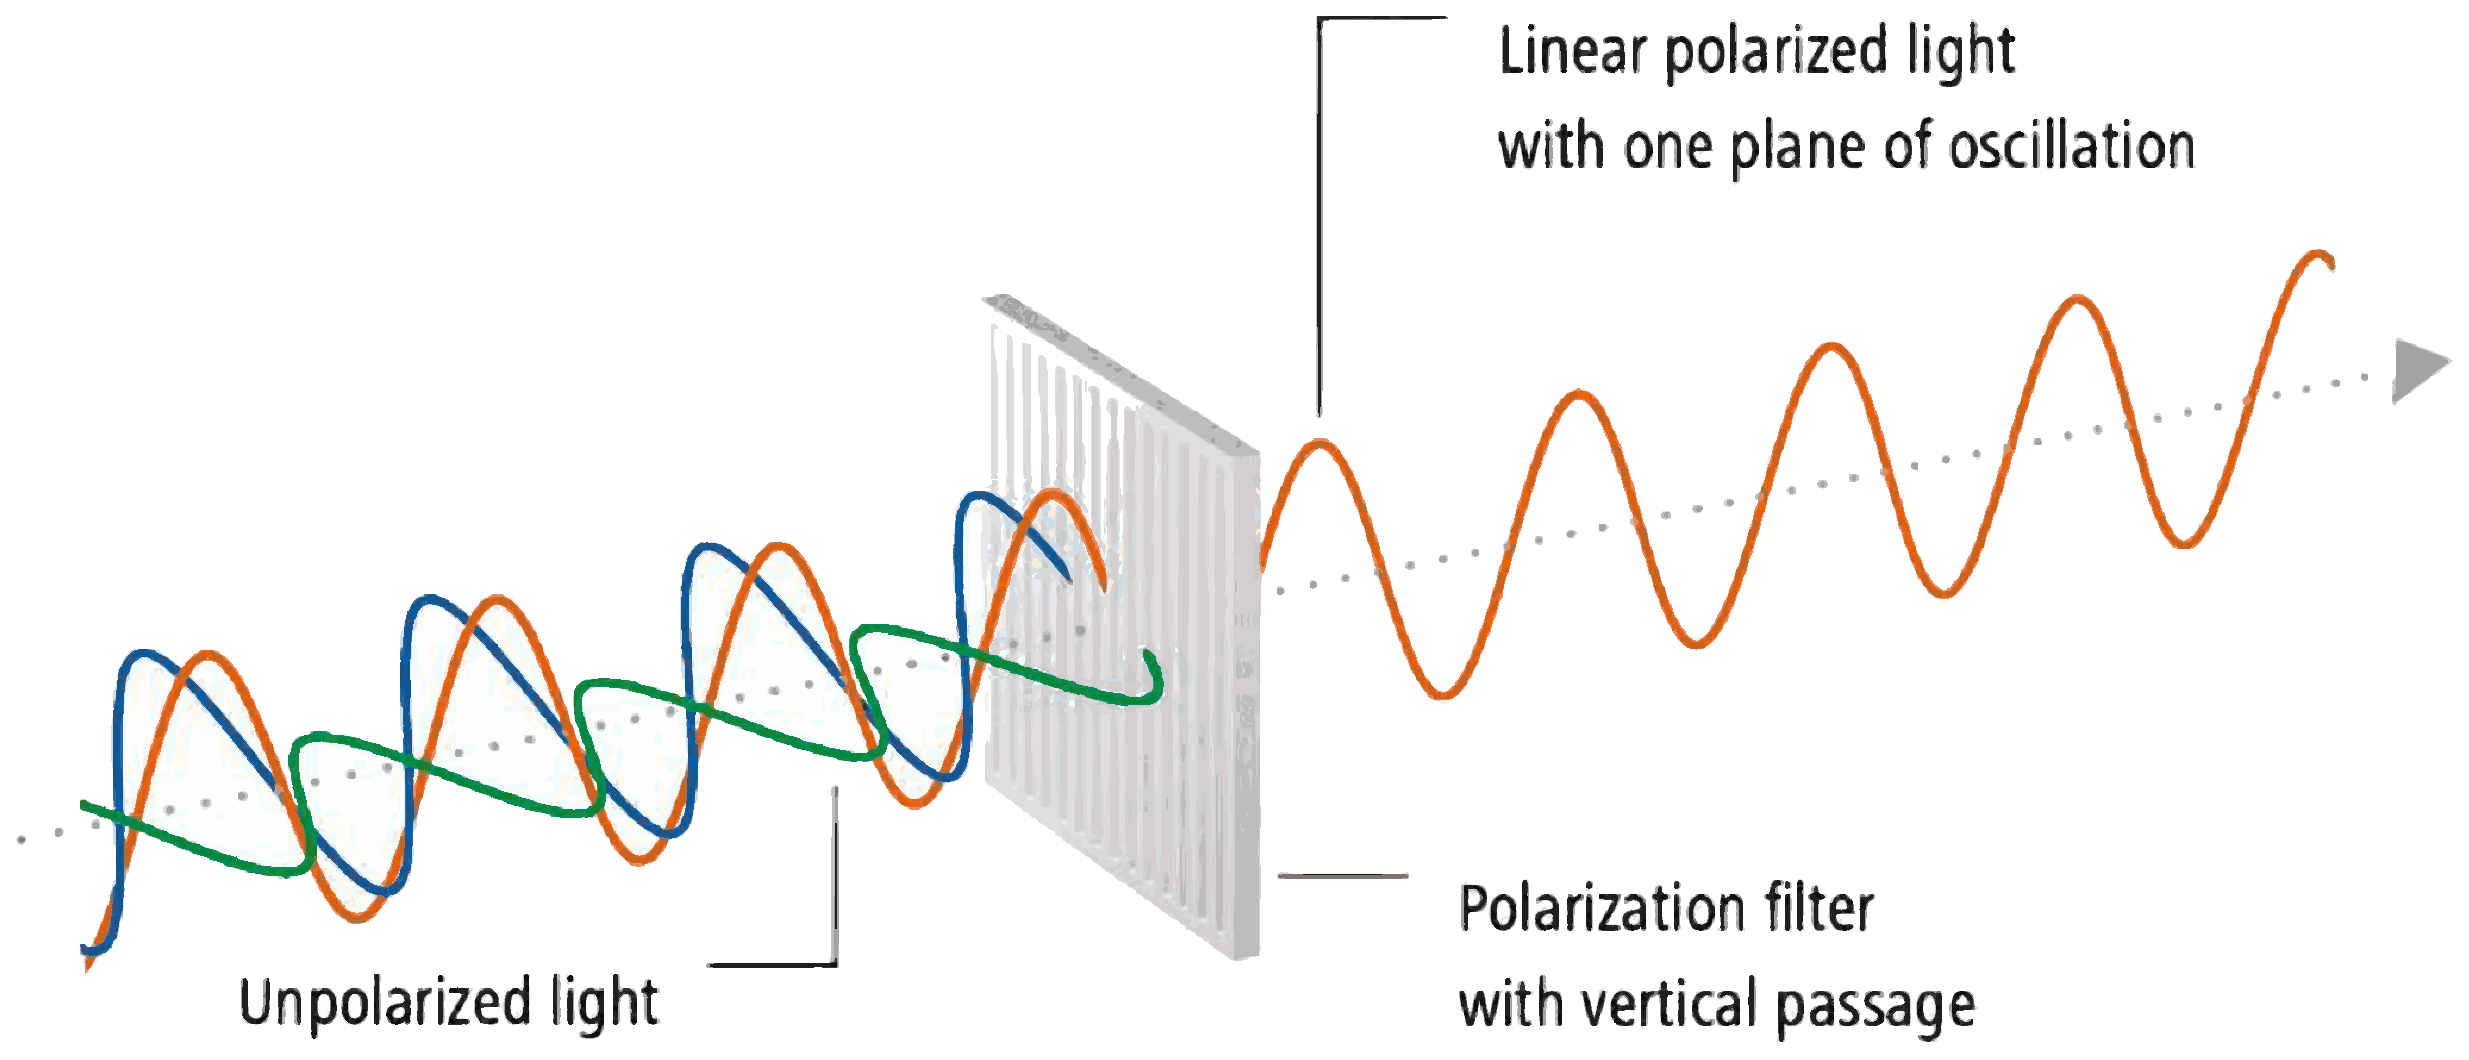
\includegraphics[width=0.6\linewidth]{img/Unpolarized.eps}
    \caption{Unpolarized light passing through a polarizer and becoming linearly polarized light.}
    \label{fig:unpolarized}
    \nocite{unpolarized}
\end{figure}

Now, let's consider the superposition of two perpendicular waves. The vector addition of these waves give a resultant vector at 45°
\begin{figure}[!phbt]
    \centering
    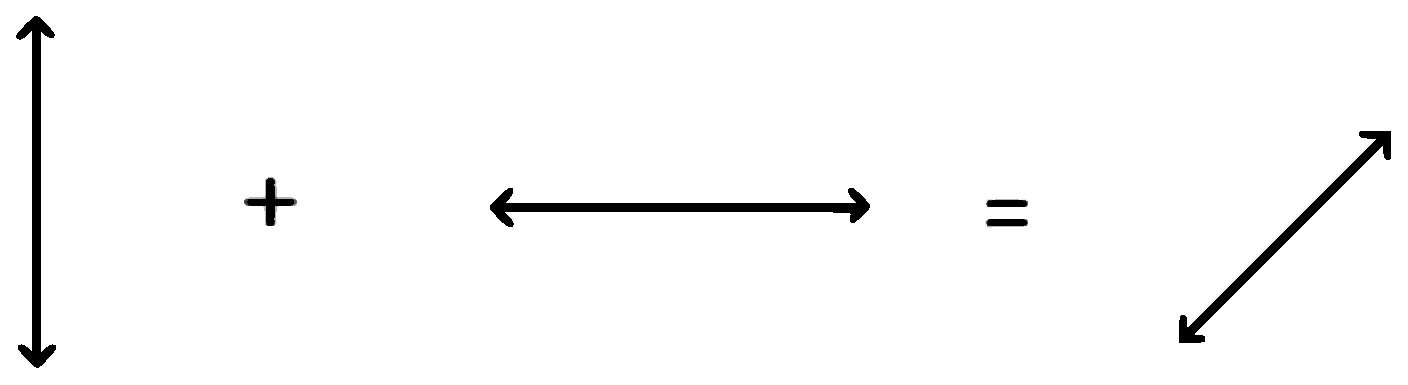
\includegraphics[width=0.5\linewidth]{img/45polarized.eps}
    \caption{Vertically linearly polarized light plus Horizontally polarized light give you polarized light at a 45° angle.}
    \label{fig:45polarized}
\end{figure}
We can quickly see that our polarized light can be thought of a superposition of many E-fields that give a resultant vector.

For the resultant vector in fig. \ref{fig:45polarized} to be linearly polarized that means that the vertically polarized light and the horizontally polarized light have to be in \hl{phase} with eachother. That is if we have two waves, $U_1 = E_0e^{kz-wt + \phi_1}$ and $U_2 = E_0e^{kz-wt + \phi_2}$ then
\begin{equation*}
    \phi_1 = \phi_2
\end{equation*}
Which means the electric fields oscillate together--reaching maximums and minimums at the same time.

Should $\phi_1 \neq \phi_2$ we get what is called elliptically polarized light with the special case of circularly polarized light.

Unfortunately, it is nearly impossible to get a visual representation of this without animations, so I will be recommending you to visit the video "Some light quantum mechanics (with minutephysics)" by 3Blue1Brown and skip to four minutes into the video to get a good visualization of this concept.
\\
\
\\
\begin{figure}[!phbt]
    \centering
    \href{https://youtu.be/MzRCDLre1b4}{
        \scalebox{0.9}{
            \parbox{\textwidth}{
                \centering
                \textbf{3Blue1Brown video to visualize polarization}\\
                \vspace{3mm}
                \includegraphics[width=\linewidth]{img/3b1b.eps}}
        }
    }
\end{figure}

Now, we should have a pretty decent understanding of polarization and should be able to understand this figure.
\begin{figure}[!phbt]
    \centering
    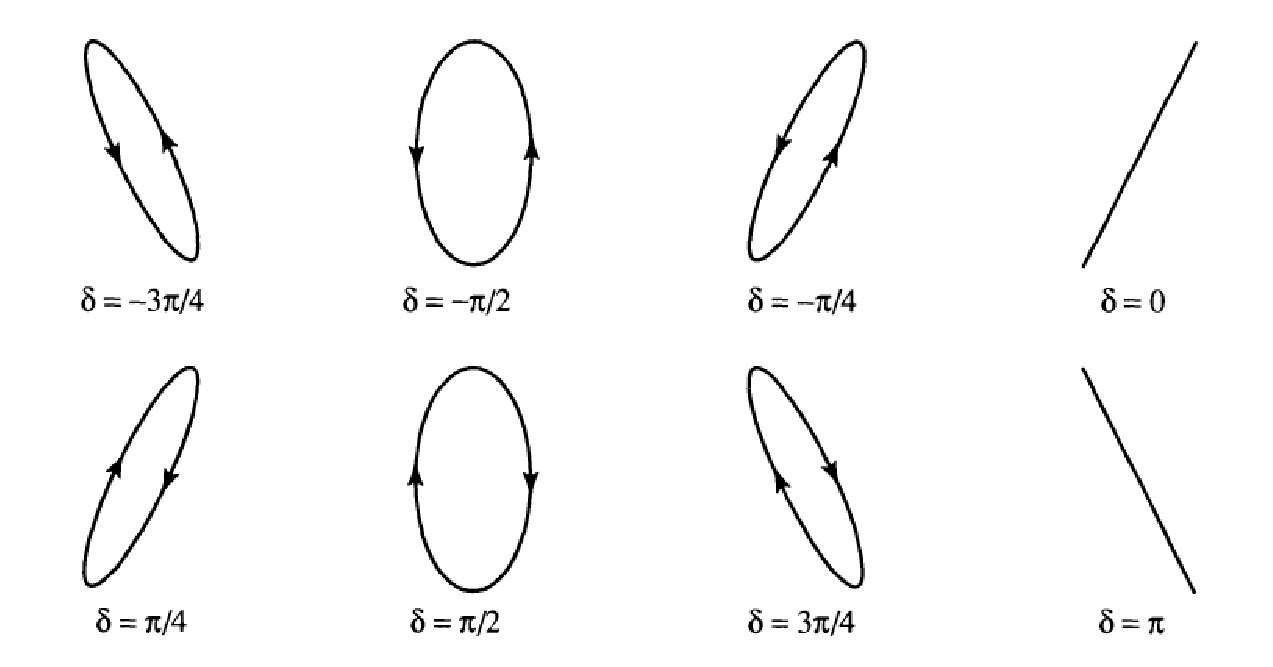
\includegraphics[width=0.55\linewidth]{img/polarpolarization.eps}
    \caption{Phase differences and their resultant vectors}
    \label{fig:polarpolarization}
\end{figure}

When two polarizers are orthogonal in their polarizing direction we call them \hl{crossed polarizers}, it should be trivial that these polarizers do not let any light through.
\\
We notice we have left-circularly polarized light and right-circularly polarized light that will be depicted by $\mathcal{L}$ and $\mathcal{R}$ respectively.
If we extend the idea of superposition to this $\mathcal{L}$ and $\mathcal{R}$ polarized light we can see that
\begin{figure}[!phbt]
    \centering
    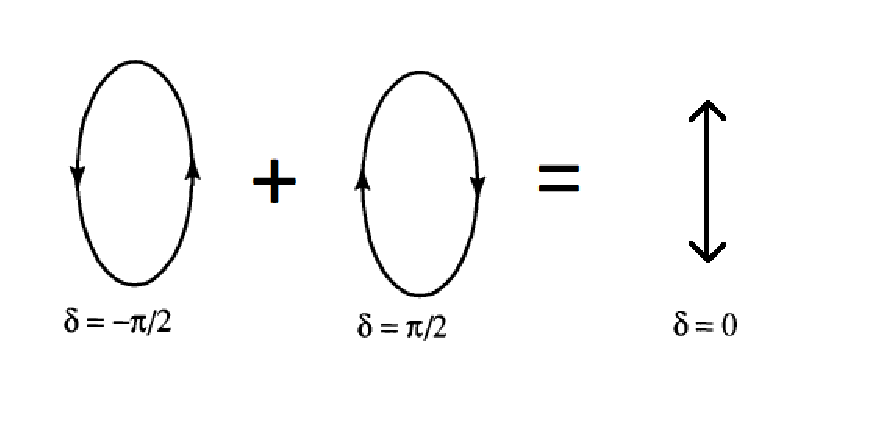
\includegraphics[width=0.5\linewidth]{img/leftright.eps}
    \caption{Adding left and right circularly polarized light gives you linearly polarized light.}
    \label{fig:leftright}
\end{figure}
\\
Which leads to an interesting way of explaining optical activity.

\subsection{Wave-plates and Optical activity}
Eventually you will hear the terms quarter-wave plates, half-wave plates, and optical activity.
Some materials, like twisted nematic crystals seem to have a different index of refraction for light depending on whether it is $\mathcal{L}$-polarized or $\mathcal{R}$-polarized. Taking in mind fig. \ref{fig:leftright} we can come to the conclusion that this will cause a rotation in the linear polarization of light and is called \hl{optical activity}.

\begin{figure}[!phbt]
    \centering
    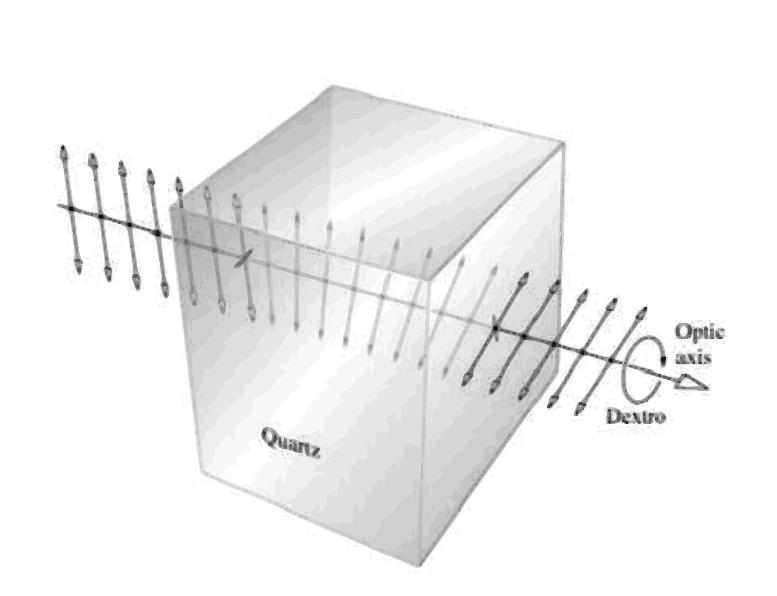
\includegraphics[width=0.4\linewidth]{img/opticalactivity.eps}
    \caption{Linearly polarized light passing through a quartz and being rotated due to optical activity}
    \label{fig:opticalactivity}
\end{figure}

Wave plates are \hl{birefringent} materials that have a slow or fast axis causing a phase difference in the superposition of light. This converts linearly polarized light into elliptically polarized light. A half-wave plate imposes a half wavelength difference or a $\pi$ phase difference while a quarter wave plate imposes a quarter wavelength difference or a $\pi/2$ phase difference.
\\
\\
Quarter wave plates convert linearly polarized light into circularly polarized light, while half wave plates rotate the linear polarization of light by 90°

\begin{figure}[!phbt]
\begin{minipage}{0.5\linewidth}
    \centering
    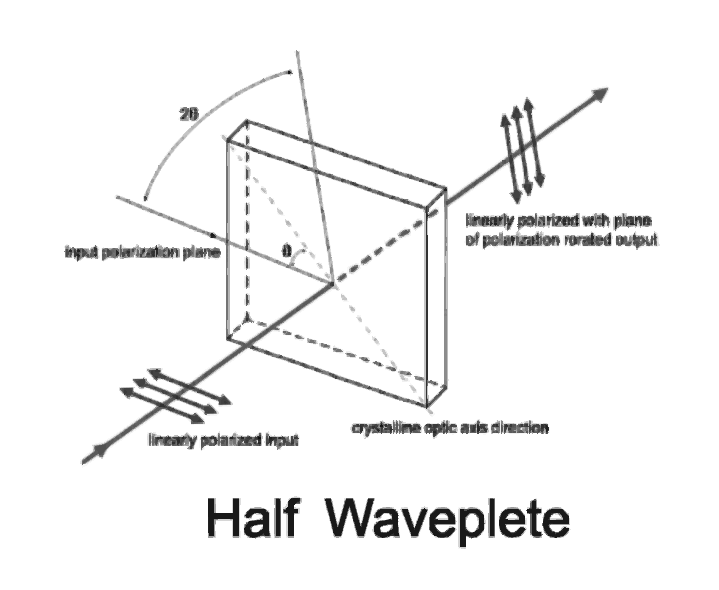
\includegraphics[width=\linewidth]{img/halfwp.eps}
    \caption{Half-wave plate rotating linearly\\ polarized light 90°}
    \label{fig:halfwp}
\end{minipage}
\begin{minipage}{0.5\linewidth}
    \centering
    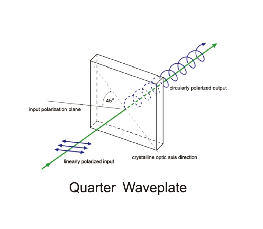
\includegraphics[width=\linewidth]{img/quarterwp.eps}
    \caption{Quarter wave plate converting linearly polarized light to circularly polarized light}
    \label{fig:quarterwp}
\end{minipage}
\end{figure}

\pagebreak
%--------------------------------------------------------------------------------------------------------------------------------%
\section{Fourier Optics}
Before starting this section, familiarize yourself with Fourier analysis and the Fourier Transform.
\subsection{The double slit experiment}
Knowing that light exhibit wave-particle duality is quite useful in explaining the phenomena of the double slit experiment shown below.

\begin{figure}[!phtb]
    \centering
    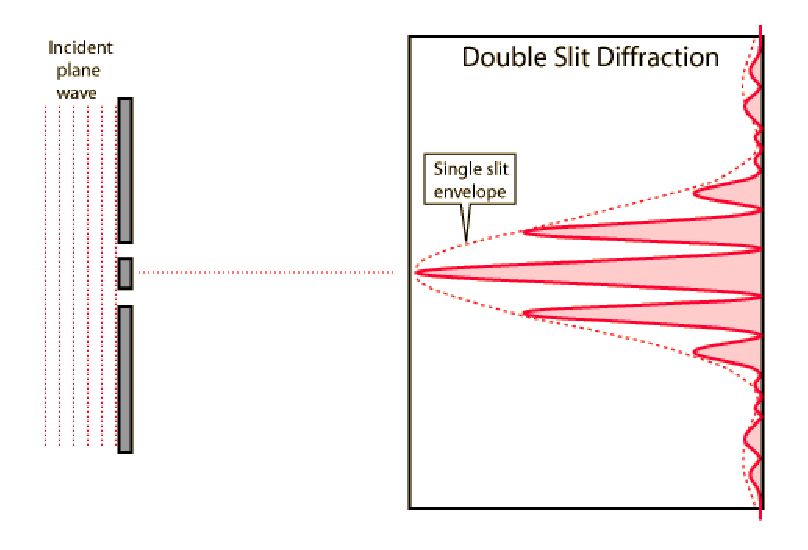
\includegraphics[width=0.5\linewidth]{img/Double_Slit.eps}
    \caption{Shining light through a double slit and getting an interference pattern}
    \label{fig:double_slit}
\end{figure}

Using the knowledge of the previous chapters, it should be trivial as to why there exists a double slit diffraction pattern. This is a result of the interference of light when it is acting as a wave.

Now, what about below:
\begin{figure}[!phbt]
    \centering
    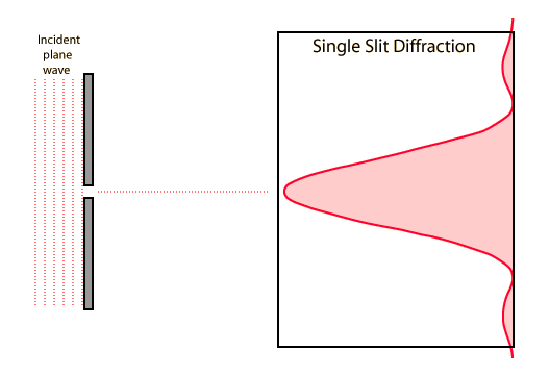
\includegraphics[width=0.5\linewidth]{img/Single_Slit.eps}
    \caption{Interference pattern emerging from a single slit}
    \label{fig:single_slit}
\end{figure}

Take a second to think about this and try to come up with some explanation as to why this occurs.
\\
\pagebreak
\\
As we described in Lemma \ref{superposition_lemma}, the superposition of waves give you a valid solution to the wave equation. Let's take a look at Huygens principle:
\begin{figure}[!phbt]
    \centering
    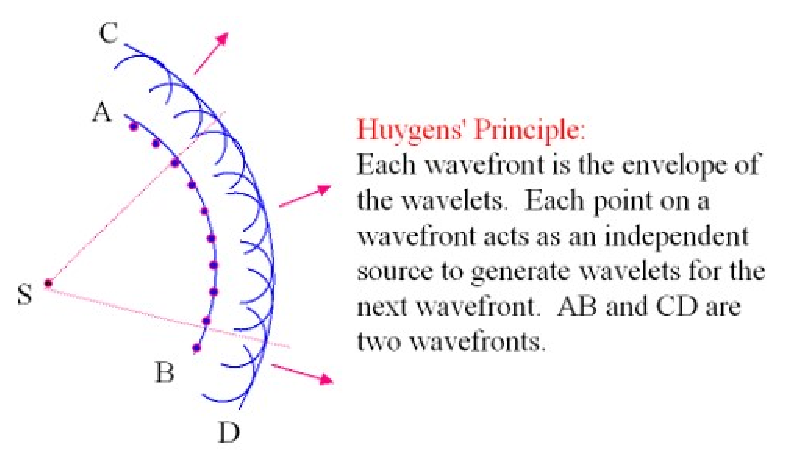
\includegraphics[width=0.5\linewidth]{img/Huygens.eps}
    \caption{Superposition principle of wavelets superimposing to create the wave-front}
    \label{fig:huygens}
\end{figure}
\\
Now with this idea, it should be clear to see why the single slit creates an interference pattern. By blocking some of the wavelets in the original wavefront you will get a different wavefront resulting from interference.
\\
\\
Now, exactly how do we calculate this diffraction pattern that is created from the single or double slit? Well, turns out if we think of the slit as infinitesimally small slits we can actually calculate the diffraction pattern the same way as we would the double slit: using a bit of vector calculus. For the purposes of this book, the math proceeding this will be hand-wavy however, I do encourage you to reference \cite{MIT} and \cite{fourier} or \cite{hecht_2017}.
\\
\\
We can represent a plane wave propagating through a slit using Huygens' principle as spherical waves propagating from the source of infinitesimal slits with width = $b-a$
\begin{equation}
    E(r,z) = \int_a^b E_0 \frac{e^{ikr}}{r} dz
\end{equation}
Referencing "Introduction to Fourier optics" by Joseph W. Goodman \cite{fourier},

Throw in some approximations and this eventually becomes,
\begin{equation}
    E(r,z) = E_0 \int_a^b e^{-ik_z z} dz
\end{equation}
Which looks a lot like the Fourier transform. Using an aperture function g(x) we can extend the integral from $-\infty$ to $\infty$ and replace it with the Fourier transform of g(x).
\begin{equation}
    E(r,z) = E_0 \int_{-\infty}^\infty g(x) e^{-ik_z z} dz = E_0\mathcal{F}(g(x))
\end{equation}

The aperture function can be used to represent our slit, say we have a slit of width $\alpha$
\begin{figure}[!phbt]
    \centering
    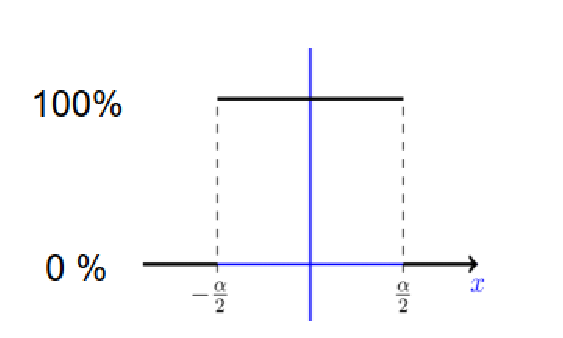
\includegraphics[width=0.4\linewidth]{img/Aperture.eps}
    \caption{Aperture function of a slit with width $\alpha$, y-axis represents transmittance of light.}
    \label{fig:aperture}
\end{figure}
\\
Obtaining the Fourier transform of fig. \ref{fig:aperture} and squaring it will give you an intensity distribution of 
\begin{equation}
    I = I_0 \frac{sin^2(\frac{k_z\alpha}{2})}{(k_z\alpha)^2} = sinc^2(\phi/2)
\end{equation}
Which is exactly what is observed in experiment.
\subsection{Lens as a phase transformation}
 The concept of the lens as a phase transformation should not be foreign to you, in fig. \ref{fig:planarwave} we saw the planar wave being transformed into a spherical wave.
 Well, turns out we can think of every type of interaction of light with matter as an amplitude and phase transformation. Not only that, but we can think of them as \hl{linear transformations}
 That is, if we have a wave $U(r)$ the linear multiplication of a transformation $t(r)$ results in a wave $U'(r)$, that is:
 \begin{equation}
     U'(r) = t(r)U(r)
 \end{equation}
 
The phase transformation of a thin lens for example is
 \begin{equation}
     t_l(r) = e^{-ikr/2f}
 \end{equation}
where f is the focal length of the lens.
 
\subsection{Fourier transforming properties of a lens}
Arguably, one of the most important aspects of Fourier optics is that of the Fourier transforming properties of a lens.

Turns out you can quite simply obtain the Fourier transform of an optical input, all you must do is use a lens and place it in any of the following configurations:

\begin{figure}[!phbt]
    \centering
    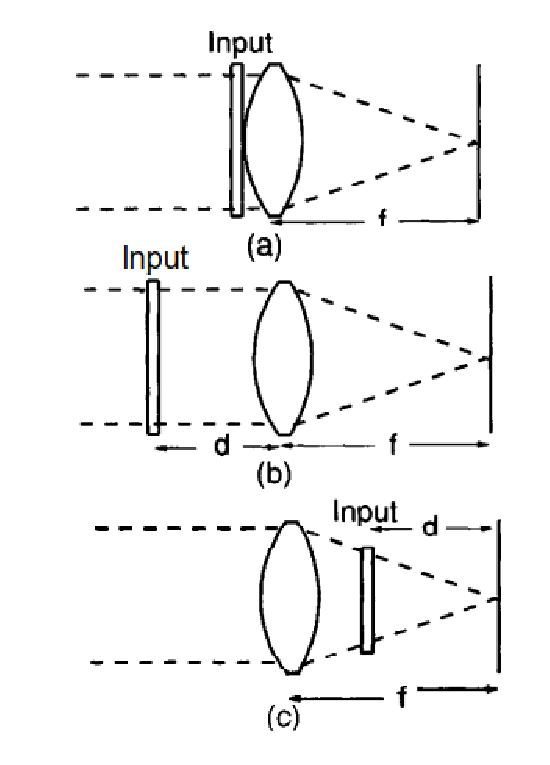
\includegraphics[width=0.4\linewidth]{img/fouriertrans.eps}
    \caption{Three configurations (a)(b)(c) of obtaining a optical Fourier transform of an input.}
    \label{fig:fouriertrans}
\end{figure}

I would recommend to reference \cite{fourier} again.

In summary, it is only in the special case of configuration fig. \ref{fig:fouriertrans} (b) where d = f that we see an exact Fourier transform relation:
\begin{equation}
U'(x,y) = \frac{A}{i\lambda f} \iint_{-\infty}^{\infty} U(x,y) e^{-i\frac{2\pi}{\lambda f}(xu+yv)} dudv = \frac{A}{i\lambda f} \mathcal{F}(U(x,y))
\end{equation}
In most other cases we have a quadratic phase factor of the form $e^{i\frac{k}{2f}(x^2+y^2)}$ preceding the integral. If we just want the intensity of the beam however, this phase factor does not matter. (eq. \ref{Intensity})

\pagebreak

\subsection{The 4-f correlator}

\begin{figure}[!phbt]
    \centering
    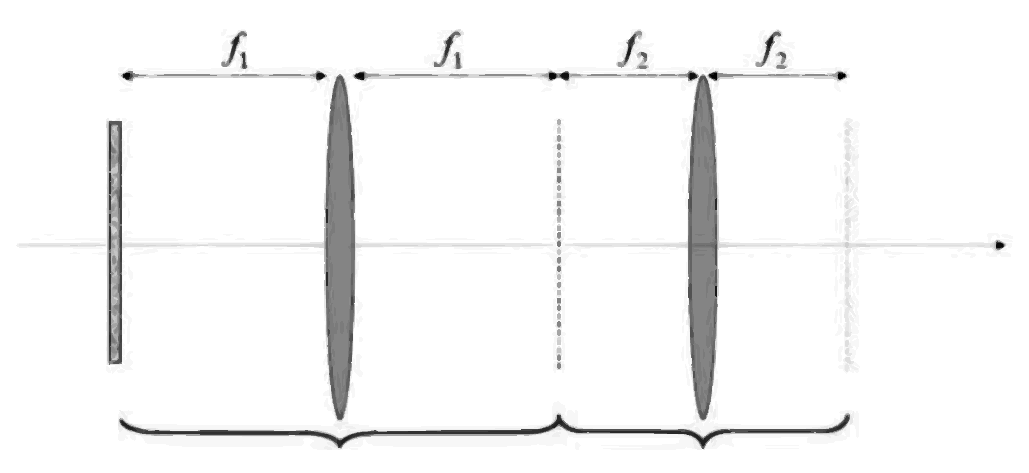
\includegraphics[width=0.6\linewidth]{img/4f_correlator.eps}
    \caption{4f system with the Fourier plane in the center.}
    \label{fig:4f_correlator}
\end{figure}

The 4-f correlator is a system which allows filtering in the Fourier plane of the object. In fig. \ref{fig:4f_correlator} we can place an object to the left of the first lens with focal length $f_1$. To the right of the lens we will get the Fourier transform of that object. This plane is called the Fourier plane and can be used to apply filters in the frequency domain. Since the second lens has a focal length $f_2$ and is a distance $f_2$ away from the Fourier plane, it is expected to get the original object.
\\
This is a useful setup when you want to apply filters to your object in the frequency domain and then image that object.


%--------------------------------------------------------------------------------------------------------------------------------%
\section{Spatial Light Modulators (SLM)}
Now we have all the theoretical tools to explain how a spatial light modulator functions.

\subsection{Twisted Nematic Crystals and the SLM}
Twisted Nematic Crystals are crystals that exhibit optical activity. Additionally, they orient themselves based on an electric field giving great control of a wavefront.

\begin{figure}[!phbt]
    \centering
    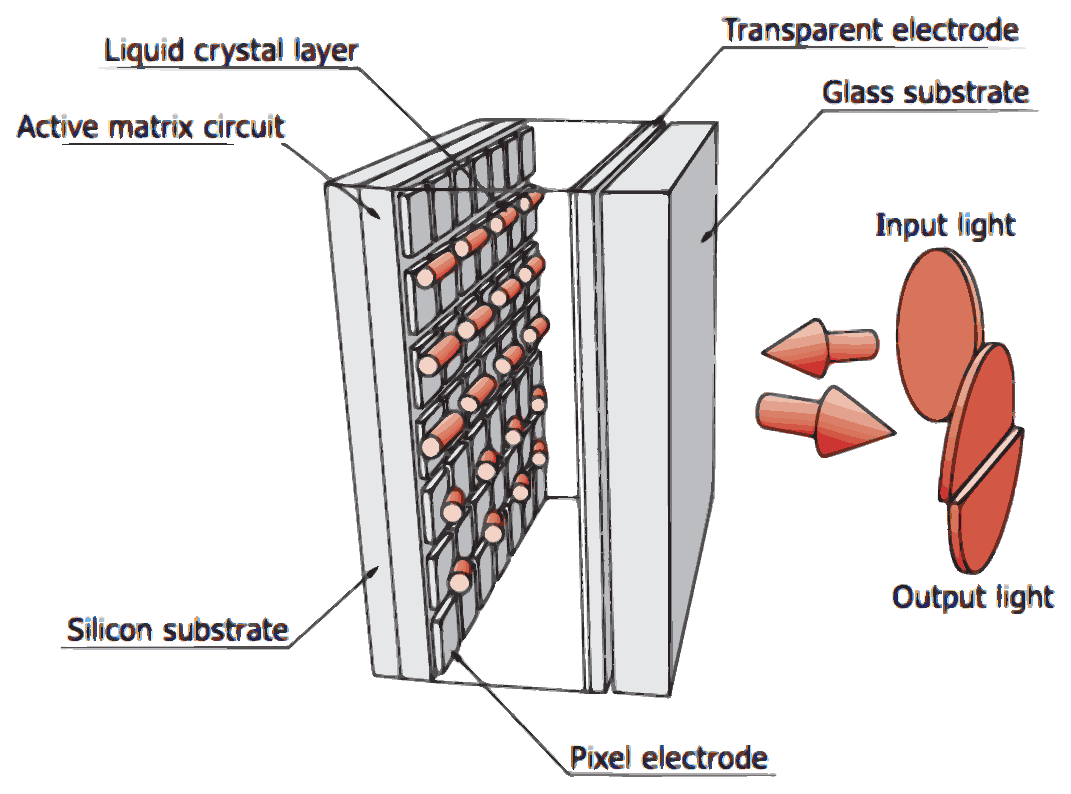
\includegraphics[width=0.6\linewidth]{img/twistedcrystals.eps}
    \caption{Diagram of how an SLM is structured.}
    \label{fig:twistedcrystals}
\end{figure}

Since optical activity is orientation dependent by creating a liquid crystal layer and selectively inducing optical activity, it is possible to induce selective polarization changes which in turn induce interference and changes the wavefront.

\pagebreak
\subsection{Gerchberg-Saxton Algorithm}
The Gerchberg-Saxton Algorithm is a iterative algorithm useful in finding the phase mask of a target image.

In Fourier analysis we learn that a signal can be broken into two parts, the magnitude and the phase. An image is a 2-D signal and can be split into these two parts by calculating the 2-D Fourier transform of the source image.

\begin{figure}[!phbt]
\centering
	\begin{minipage}{.3\linewidth}
		\centering
    	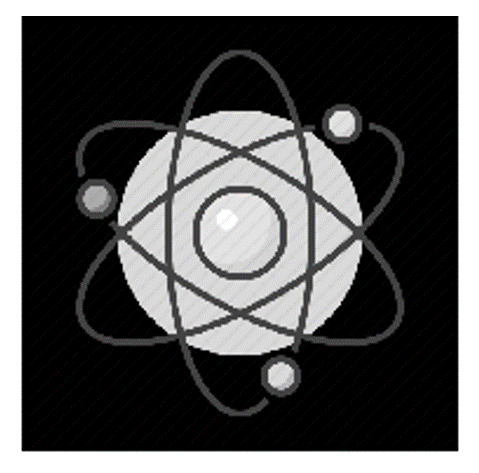
\includegraphics[width= \linewidth]{img/sourceimage.eps}
    	\caption{Source image}
    	\label{fig:sourceimage}
    \end{minipage}
    \begin{minipage}{.3\linewidth}
    	\centering
    	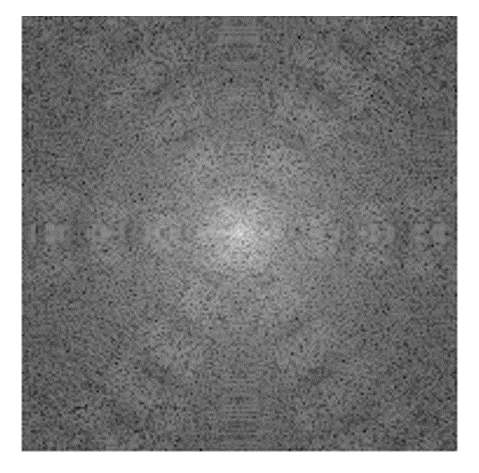
\includegraphics[width= \linewidth]{img/magnitudeimage.eps}
    	\caption{Magnitude of source}
    	\label{fig:magnitudeimage}
    \end{minipage}
    \begin{minipage}{.3\linewidth}
    	\centering
    	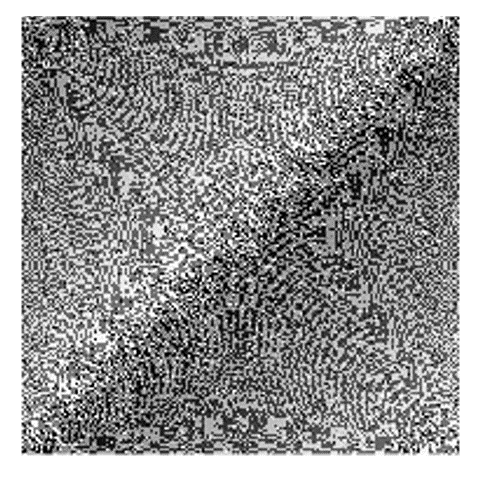
\includegraphics[width= \linewidth]{img/phaseimage.eps}
    	\caption{Phase of source}
    	\label{fig:phaseimage}
    \end{minipage}
\end{figure}

What happens when we try to get the original image only using one of the parts? Running the inverse Fourier transform of the magnitude or the phase gives us:
\begin{figure}[!phbt]
\centering
	\begin{minipage}{.45\linewidth}
		\centering
    	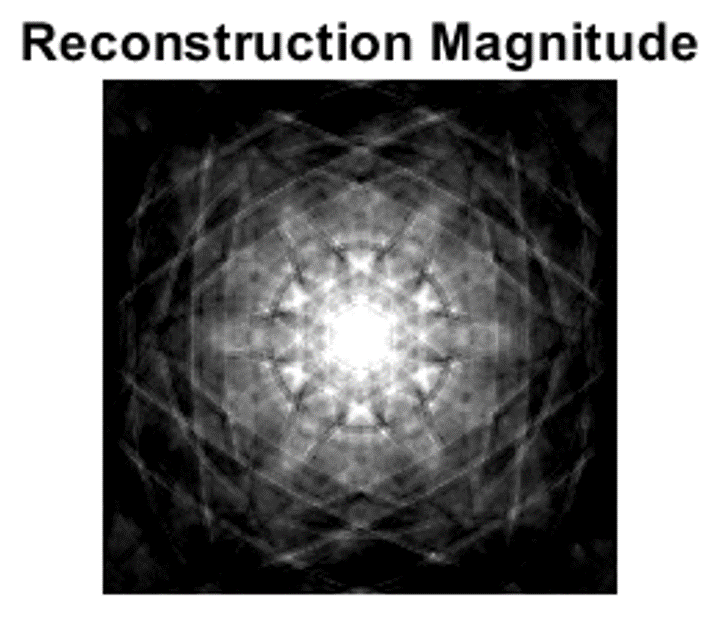
\includegraphics[width= 0.92\linewidth]{img/magnituderecon.eps}
    	\caption{Reconstruction only using the magnitude}
    	\label{fig:magnituderecon}
    \end{minipage}
    \begin{minipage}{.45\linewidth}
    	\centering
    	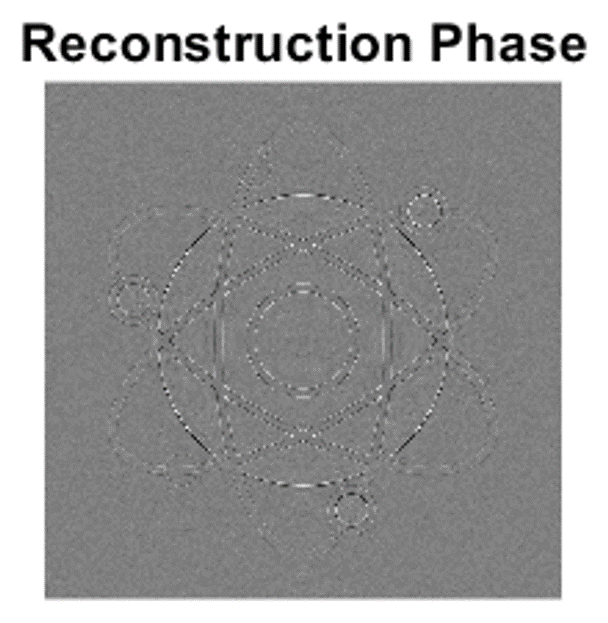
\includegraphics[width= 0.8\linewidth]{img/phaserecon.eps}
    	\caption{Reconstruction only using the phase}
    	\label{fig:phaserecon}
    \end{minipage}
\end{figure}

Arguably the phase information is more important than the magnitude information. The phase information reconstructs the original image but, lacks intensity information.
It is possible to modify the phase information in such a way that the image becomes clearer by optimizing the intensity of the reconstruction. This can be done by using an iterative phase algorithm such as the Gerchberg-Saxton algorithm. Alg. \ref{alg:gerchberg-saxton}


\begin{algorithm}[H]
\caption{Gerchberg-Saxton algorithm}\label{alg:gerchberg-saxton}
\begin{algorithmic}[1]
\Procedure{Gerchberg-Saxton}{$source,target$}\\
\Comment{Fast Fourier transform of target}
\State A $\equiv$ FFT(target)\\
\Comment{Replace modulus of A with source.}
\State $B\equiv$ Amplitude(source)$\times e^{i\times Phase(A)}$ \\
\Comment Inverse Fourier transform B
\State $C\equiv$ IFT(B) \\
\Comment{Modulus of target with generated phase of C}
\State $D\equiv$ Amplitude(target)$\times e^{i \times Phase(C)}$ \\
\State $A\equiv$ FFT(D)

\State \textbf{return} $A$ \\\Comment{Repeated until error is small}
\EndProcedure

\end{algorithmic}

\end{algorithm}

Time to put this all together now,
Let us calculate the phase mask of a target image and feed it to the SLM so that our light is now encoded with this phase mask.
Next, let's pass our light through a lens and get the Fourier transform of that light; what we should see is the original target image. This process of reconstructing images is the basics of \hl{holography}.
\begin{figure}[!phbt]
\begin{minipage}{0.45\linewidth}
    \centering
    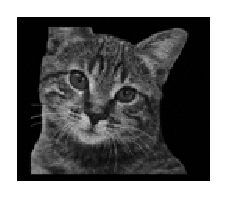
\includegraphics[width=\linewidth]{img/cat1.eps}
\end{minipage}\hfil
\begin{minipage}{0.45\linewidth}
    \centering
    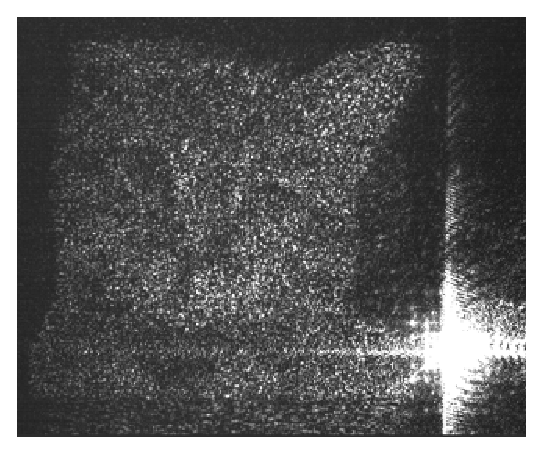
\includegraphics[width=\linewidth]{img/cat2.eps}
\end{minipage}
\caption{A cat reconstructed by using the Gerchberg-Saxton algorithm with the zeroth order on the bottom right.}
\label{fig:catrecon}
\end{figure}

\begin{figure}[!phbt]
\begin{minipage}{0.45\linewidth}
    \centering
    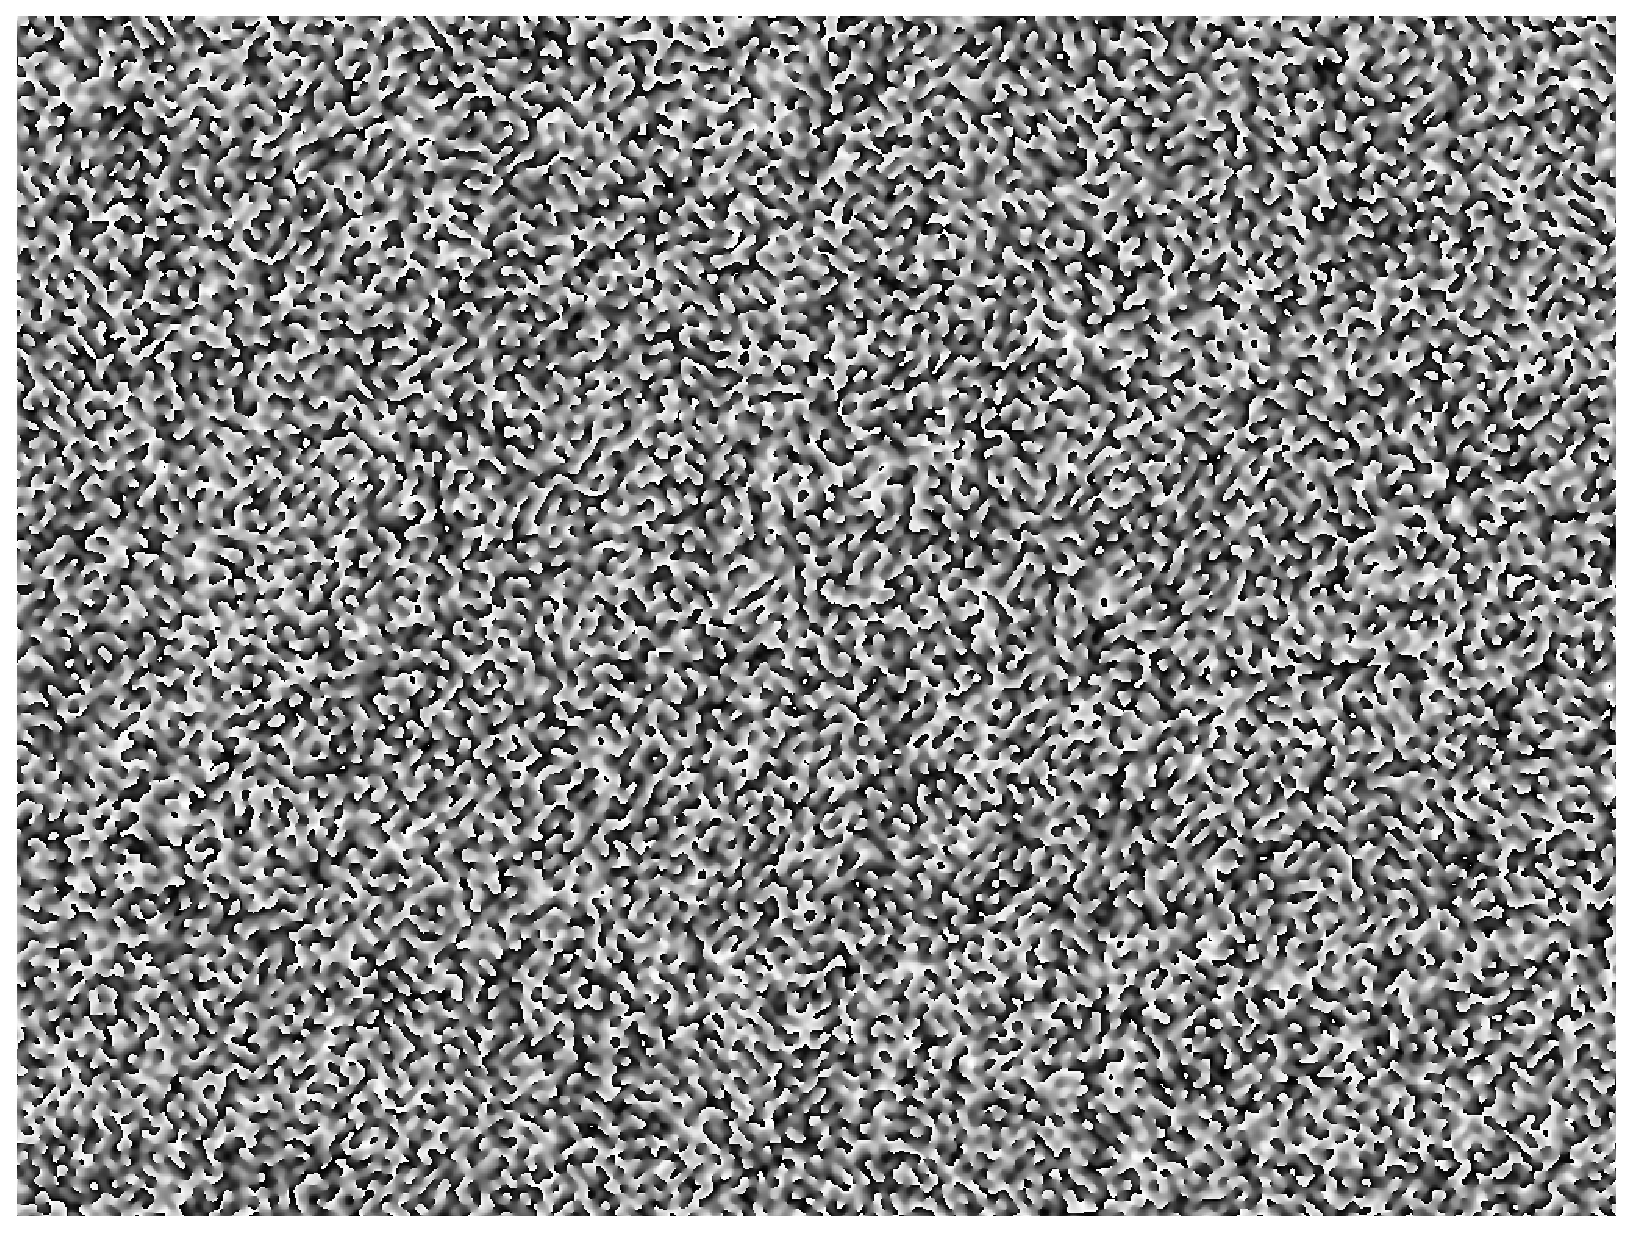
\includegraphics[width=\linewidth]{img/QR1.eps}
\end{minipage}\hfil
\begin{minipage}{0.45\linewidth}
    \centering
    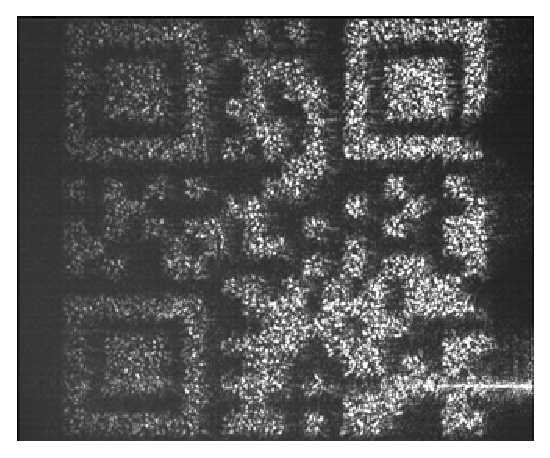
\includegraphics[width=\linewidth]{img/QR2.eps}
\end{minipage}
\caption{A phase mask generated by the Gerchberg-Saxton algorithm and its reconstructed image.}
\label{fig:qrcoderecon}
\end{figure}


\subsection{All-Optical Neural Networks}
What we described previously is a transformation from frequency space to temporal space. Generating an image from the phase information of that image.
A neural network is nothing more than a transformation from input space to output space.

\begin{figure}[!phbt]
    \centering
    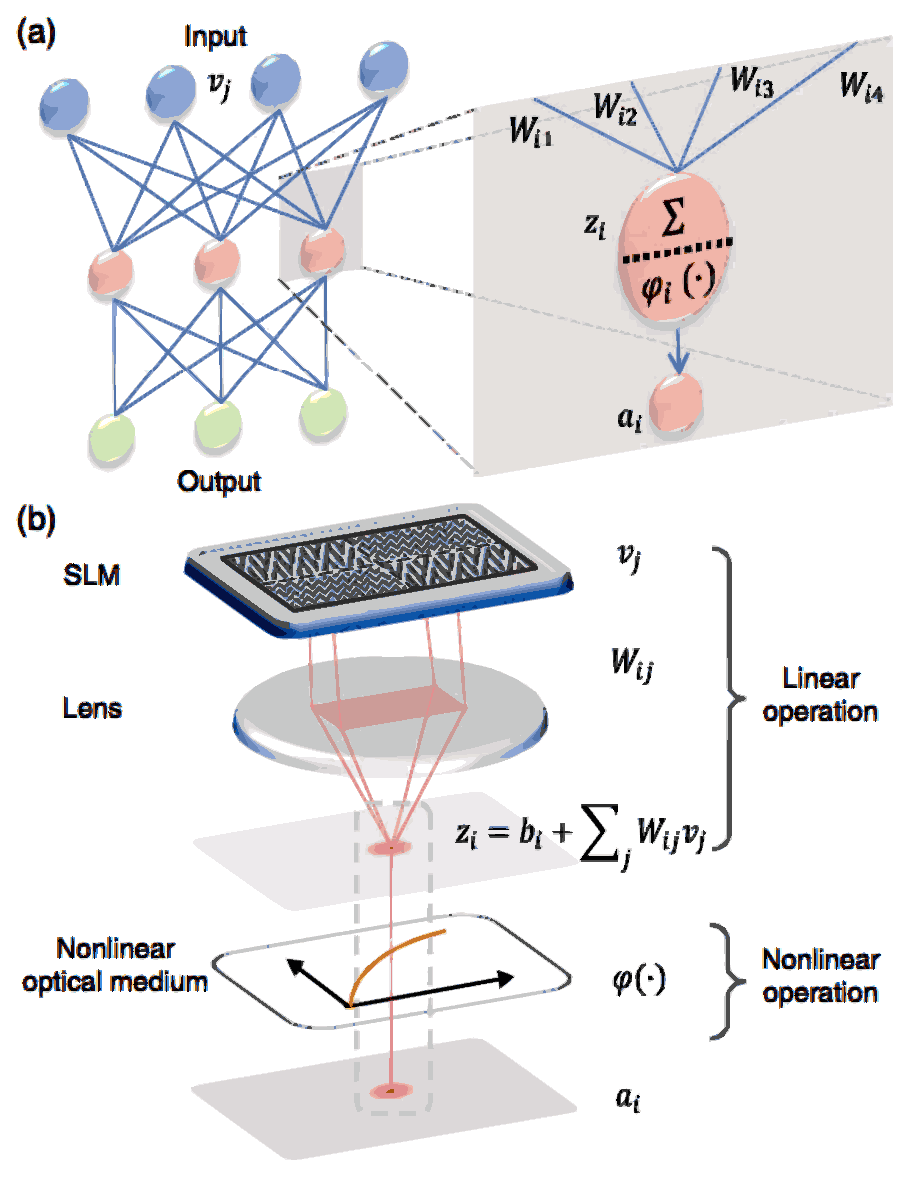
\includegraphics[width=0.55\linewidth]{img/AONN.eps}
    \caption{In (a) the theoretical design of a Neural network is presented, in (b) the optical implementation is represented}
    \label{fig:AONN}
\end{figure}

A neural network is split into two parts, a linear operation and a nonlinear operation.
I recommend watching another 3B1B video in order to understand neural networks. Further, I recommend reading \cite{AONNHongKong}.
\begin{figure}[!phbt]
    \centering
    \href{https://youtu.be/aircAruvnKk}{
        \scalebox{0.8}{
            \parbox{\textwidth}{
                \centering
                \textbf{3Blue1Brown video to understand neural networks}\\
                \vspace{3mm}
                \includegraphics[width=\linewidth]{img/3b1b2.eps}}
        }
    }
\end{figure}

%--------------------------------------------------------------------------------------------------------------------------------%
\section{Nonlinear Optics}
Imagine bringing a cup of ice into a big hot room, obviously the temperature of the room will not change. However, bring in a truckload of ice into the room and now you will start to notice a change in temperature.
The same concept applies when we talk about high energy lasers, the energy of the beam is high enough to cause changes in the medium creating nonlinear effects.
\nocite{boyd_2020}
\subsection{Nonlinear Susceptibility}
In electromagnetism we learn that dielectric materials have an electric susceptibility tensor $\chi$, that is\footnote[1]{Under the assumption of a homogeneous, isotropic medium}:
\begin{equation}
    \textbf{P} = \epsilon_0 \chi \textbf{E}
\end{equation}
The polarization of a dielectric is parallel and proportional to the electric field.
Now, let's consider the Taylor series expansion:
\begin{equation}
    \textbf{P} = \epsilon_0 (\chi^{(1)} \textbf{E} + \chi^{(2)} \textbf{E}^2 + \chi^{(3)} \textbf{E}^3 + ..)
\end{equation}
Where $\chi^{(1)}$, $\chi^{(2)}$, and $\chi^{(3)}$ are first-order, second-order, and third-order susceptibilities, respectively.

The wave equation presented in eq. \ref{eq:waveequation} assumes a vacuum, this equation is modified to account for nonlinear mediums:

\begin{equation}
    \grad^2\textbf{E} - \frac{n^2}{c^2}\frac{\partial^2\textbf{E}}{\partial t^2} = \frac{1}{\epsilon_0 c^2}\frac{\partial^2 \textbf{P}}{\partial t^2}
\end{equation}
Which shows a dependence on the polarization $\textbf{P}$ of the medium.

Depending on the mediums atomic symmetry the susceptibility for different orders will be zero rendering many nonlinear processes unique and somewhat uncommon. For an in-depth explanation of nonlinear theory including quantum mechanics refer to Boyd \cite{boyd_2020}.
\\
\ 
\\
One should note that since we are no longer dealing with linear equations, the superposition principle described in lemma \ref{superposition_lemma} is no longer valid.

\subsection{Second-Harmonic Generation (SHG)}
Second-Harmonic Generation is a common nonlinear effect. Since all you need is a relatively cheap quartz crystal, it is often used in green laser pointers to convert red light into the output green light.

Second-Harmonic Generation is a $\chi^{(2)}$ effect and looks like:
\begin{figure}[!phbt]
    \centering
    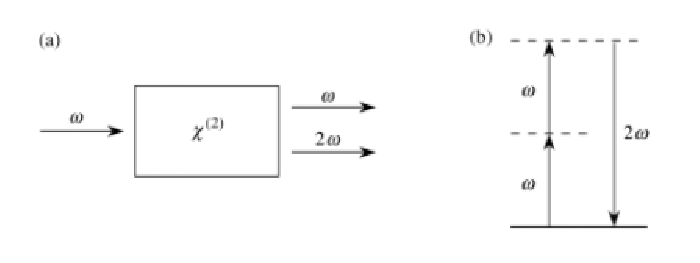
\includegraphics[width=0.55\linewidth]{img/shg.eps}
    \caption{In (a) the geometry of the process, in (b) the energy level diagram of SHG}
    \label{fig:shg}
\end{figure}

For the purposes of this text, this works in the simple case of destroying two photons of frequency $\omega$ and emitting one photon of frequency $2\omega$

This effect can be generalized for higher order harmonic generations such as third-order harmonic generation where three photons are destroyed and a photon of $3\omega$ is generated.
\pagebreak

\subsection{Spontaneous Parametric Down-Conversion (SPDC)}
Spontaneous Parametric Down-Conversion is similar to the opposite of SHG. However, this process is a bit unique.
\begin{figure}[!phbt]
    \centering
    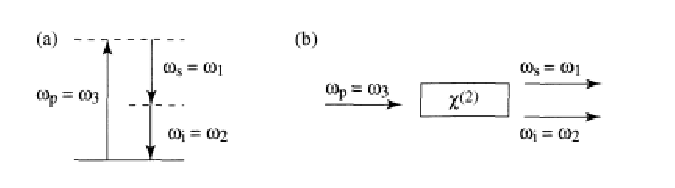
\includegraphics[width=0.65\linewidth]{img/spdc.eps}
    \caption{In (a) the geometry of the process, in (b) the energy level diagram of SPDC}
    \label{fig:spdc}
\end{figure}

Here we have two outputs, a "signal" frequency $\omega_s$ and an "idler" frequency $\omega_i$.
In the simplistic model, since we produce two photons from one we must adhere to the conservation of momentum. One of the consequences of this conservation is that the two photons produced are now correlated  in polarization (entanglement comes later), that is, if one photon has vertical polarization the other must have horizontal polarization.

\subsection{Stimulated Raman Scattering}
Stimulated Raman Scattering is a non-parametric effect meaning that the energy level of the atoms denoted by the energy level diagrams has a non-zero net effect.

\begin{figure}[!phbt]
    \centering
    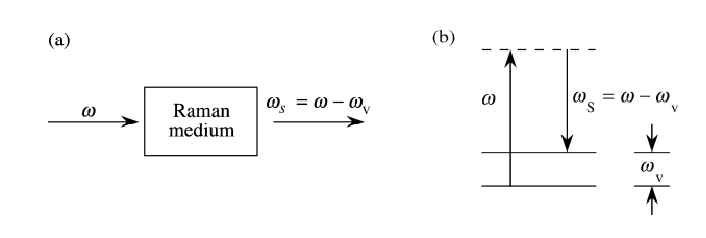
\includegraphics[width=0.65\linewidth]{img/SRS.eps}
    \caption{In (a) the geometry of the process, in (b) the energy level diagram}
    \label{fig:srs}
\end{figure}

In our simple model, this process destroys one photon of frequency $\omega$ and creates one photon with frequency $\omega_s = \omega - \omega_v$ where $\omega_v$ is the "Stokes shifted frequency". This excites a population of atoms with energy $\hbar\omega_v$. This nonlinear effect is quite useful for spectroscopy.

\subsection{Four-wave mixing}
Sum and difference nonlinear effects are quite simple and it is when you get input frequencies and get their sum or differences. Four-wave mixing is a third-order parametric process that is utilizes sum and difference effects:

\begin{figure}[!phbt]
    \centering
    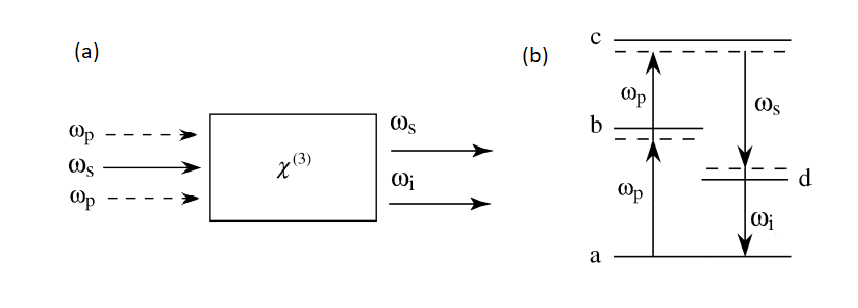
\includegraphics[width=0.65\linewidth]{img/fwm.eps}
    \caption{In (a) the geometry of the process, in (b) the energy level diagram}
    \label{fig:fwm}
\end{figure}
The pump frequencies could be the same or different, this leads to non-degenerate and degenerate cases.
FWM is a rather extensive process that the reader should research on their own.

%--------------------------------------------------------------------------------------------------------------------------------%
\section{Quantum Optics}
\subsection{Light Amplification by Stimulated Emission of Radiation}
A laser works by way of stimulated emission. This stems from Einsteins discovery of absorption and emission.
Here the Quantum theory of light assumes that photons are absorbed and emitted whenever an electron makes a jump between two quantum states. These transitions obey the conservation of energy and the frequency of the photon must satisfy:
\begin{equation}
    \hbar\omega = E_2 - E_1
\end{equation}
This automatically indicates that atoms will only absorb quantified light. This is linear optics where one photon is destroyed with frequency $\omega$ and another is created with the same frequency.

\begin{figure}[!phbt]
    \centering
    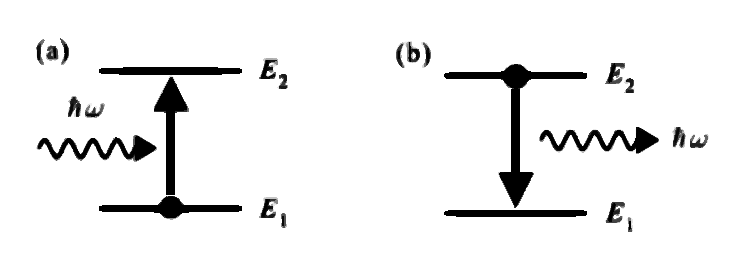
\includegraphics[width=0.65\linewidth]{img/absorption.eps}
    \caption{In (a) absorption of a photon, in (b) the spontaneous emission of a photon}
    \label{fig:absorption}
\end{figure}

Excited states will eventually drop back down and the rate at which \hl{spontaneous-emission} occurs depends on the Einstein coefficient $A$ for the transition which gives the probability distribution for spontaneous emission from $E_2$ to $E_1$ to be:
\begin{equation}
	\frac{dN_2}{dt} = -A_{21}N_2
\end{equation}
where $N_2(t)$ is the number of atoms in the excited state ($E_2$).

\hl{Absorption} also has a rate and only occurs with the right energy $\hbar\omega$ this process is not spontaneous and occurs with a rate given by the Einstein coefficient $B$. For absorption from $E_1$ to $E_2$ the rate is:
\begin{equation}
	\frac{dN_1}{dt} = -B_{12}N_1 u(\omega)
\end{equation}
Where $u(\omega)$ is the energy density of the electromagnetic field at frequency $\omega$ and $B$ depends on $\omega$.
Turns out that there's a third process that depends on the Einstein coefficient $B$ which is \hl{stimulated emission}
Stimulated emission is a quantum mechanical effect in which photons are emitted in phase with the photons that induce the transition.\cite{foxqmoptics}. The rate of stimulated emission from $E_2$ to $E_1$ is:
\begin{equation}
	\frac{dN_2}{dt} = -B_{21}N_2 u(\omega)
\end{equation}

With these concepts in mind, a laser contains a gain medium, a cavity, and an output coupler.
\begin{figure}[!phbt]
    \centering
    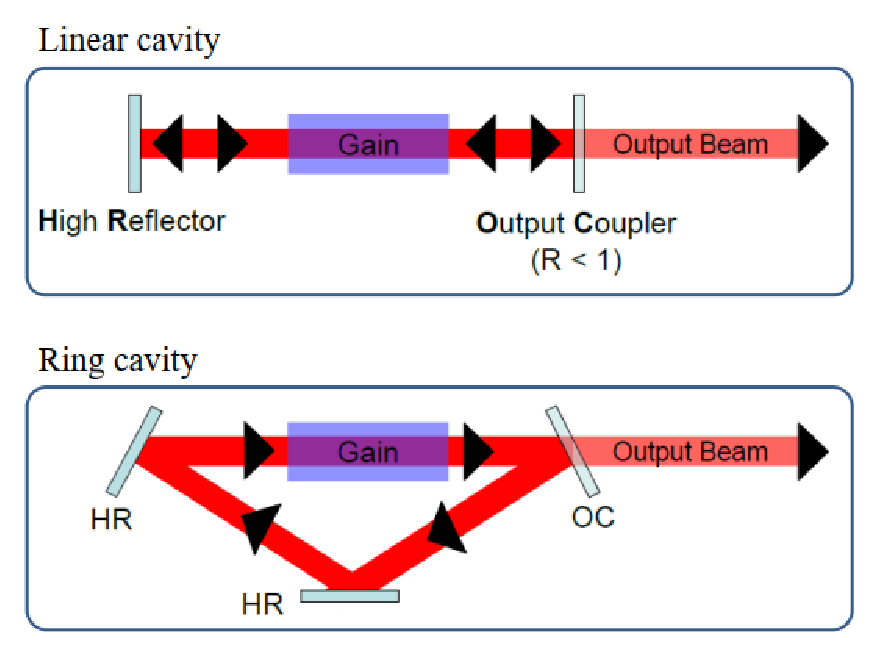
\includegraphics[width=0.65\linewidth]{img/cavity_geometries.eps}
    \caption{Two cavity geometries of many}
    \label{fig:absorption}
\end{figure}

For a laser to "lase" it the Gain has to be greater than the loss.
For the gain to be greater than the loss a condition called "population inversion" must occur, this condition states that

\begin{equation}
	N_2 > N_1
\end{equation}

When $N_2 = N_1$ this state is called the "steady state" and has the following conditions:
\\
\
\\
Gain condition:\\
	The gain is equal to the loss
\\
\
\\
Phase condition:\\

The round trip phase shift has to be zero which means that in the laser we must have a \textbf{standing wave} where the result of interference gives you a wave oscillating in amplitude but, is stationary in phase.

In the cavity these standing waves have specific frequencies that are allowed and are called \hl{modes}
\begin{equation}
	\omega_m = \frac{m\pi c}{l}
\end{equation}
The phase conditions are true when $N_2 > N_1$ as well.

Turns out that two-level systems cannot lase and at best you get the case where $N_2 = N_1$, refer to \cite{foxqmoptics},\cite{li} for more information.
\begin{figure}[!phbt]
    \centering
    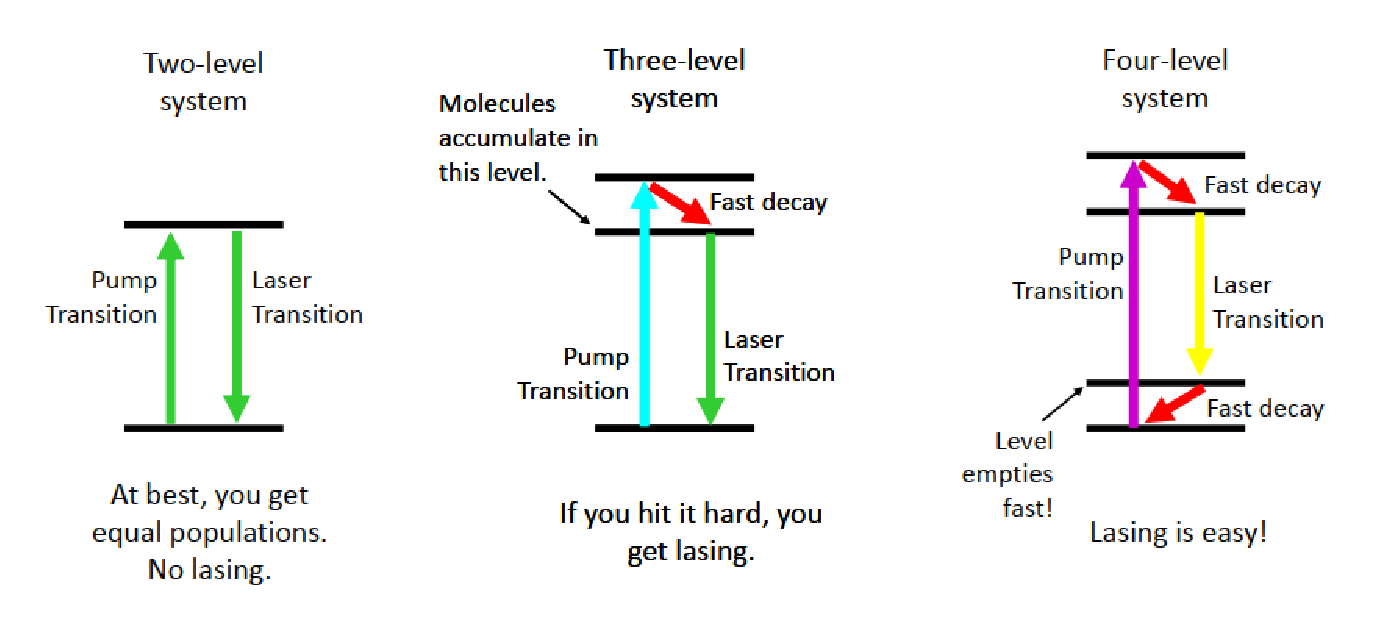
\includegraphics[width=0.75\linewidth]{img/levelsystems.eps}
    \caption{Two,Three, and Four level systems.}
    \label{fig:levelsystems}
\end{figure}

Using some nonlinear optics such as saturable absorption and mode-locking techniques it is possible to create ultrashort pulses where all the modes of the output are locked in phase with reference to each other despite having different wavelengths (imagine a fixed point on each wave being phase locked).

\subsection{Coherence}
Light can be split into three categories:
\begin{itemize}
    \item Thermal light
    \item Coherent light
    \item Pure quantum light
\end{itemize}

A great illustration by D. Gabor presents the idea of thermal and coherent light.

\begin{figure}[!phbt]
    \centering
    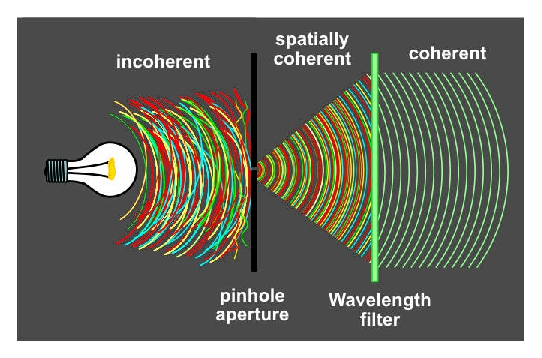
\includegraphics[width=0.65\linewidth]{img/coherence.eps}
    \caption{Starting with an incandescent light bulb (thermal light) we get spatially coherent light (mixed wavelengths) and then spatial and temporal coherent light (monochromatic).}
    \label{fig:coherence}
\end{figure}
We see that coherent light can be thought of a wave that is phase-locked and monochromatic. In other words, experiencing \hl{spatial and temporal coherence}

It's quite difficult to create a perfectly coherent source, so usually \hl{coherence time}, $\tau_c$ is considered and defined by the amount of time the phase of the wave train remains stable. \cite{foxqmoptics}

The temporal coherence of light is described by the first-order correlation function $g^{(1)}(\tau)$

\begin{equation}
    g^{(1)}(\tau) = \frac{\expval{\textbf{E}^*(t)\textbf{E}(t+\tau)}}{\expval{\abs{\textbf{E}}^2}}
\end{equation}
This is described as the degree of first-order coherence and it tells you how coherent a wavetrain is.

A more useful function however is that of second-order coherence which measures temporal coherence using intensity fluctuations.
\begin{equation}
    g^{(2)}(\tau) = \frac{\expval{\textbf{I}^*(t)\textbf{I}(t+\tau)}}{\expval{\textbf{I}(t)}\expval{\textbf{I}(t+\tau)}}
\end{equation}
We will see the applications of the second-order coherence function in describing photon statistics.

Next we will define Pure quantum light as a "single photon" source using Photon statistics.
\pagebreak
\subsection{Photon Statistics}
If we shine tiny amounts of light at a photo detector and observe the statistics of the photon counts we will see that the three different types of light sources mentioned exhibit different statistics.

\begin{figure}[!phbt]
    \centering
    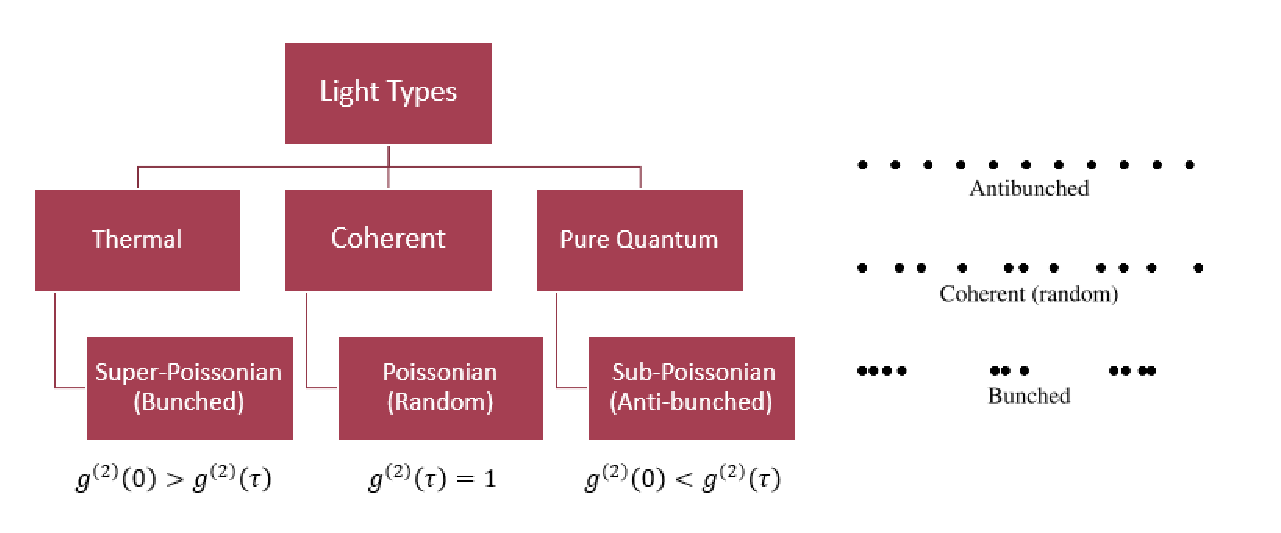
\includegraphics[width=0.85\linewidth]{img/lighttypes.eps}
    \caption{Types of light and their corresponding statistics}
    \label{fig:fwm}
\end{figure}
The bunched, random, and anti-bunched types stem from the second-order coherence function \cite{foxqmoptics}:
\begin{itemize}
    \item Bunched light: $g^{(2)}(0) > 1$
    \item Coherent light: $g^{(2)}(0) = 1$
    \item Anti-bunched light: $g^{(2)}(0) < 1$
\end{itemize}

Pure quantum light sources exhibit a quantum phenomena where it is anti-bunched, the interval of time between each photon is consistent.

This idea of anti-bunched light is the main theme of single photon sources.

\subsection{Single Photon Sources}
Spontaneous Parametric Down Conversion is quite a rare process and leads to the production of two correlated photons. This process is actually a source of single photons, however, this is a source of \hl{heralded} single photons.

They are heralded single photons because sources produce two photons and one must be detected in order to "herald" the other by way of coincidence counting.
SPDC and FWM are sources of heralded single photons and have a valuable use in Quantum Key Distribution.


%\section{Atom Trapping}
%TODO
%\section{Spectroscopy}
%TODO

%--------------------------------------------------------------------------------------------------------------------------------%
\pagebreak
\section{Signal Processing}
What are signals and how are they used?
\subsection{Analog and Digital signals}
Signals used in electronics are just changes in voltage. 
\\
An analog signal is a continuous infinite signal such as sine waves.

A digital signal is a discrete pulse such as a square wave.


https://www.tek.com/document/online/primer/xyzs-scopes/ch1/oscilloscope-basics

\begin{figure}[!phbt]
    \centering
    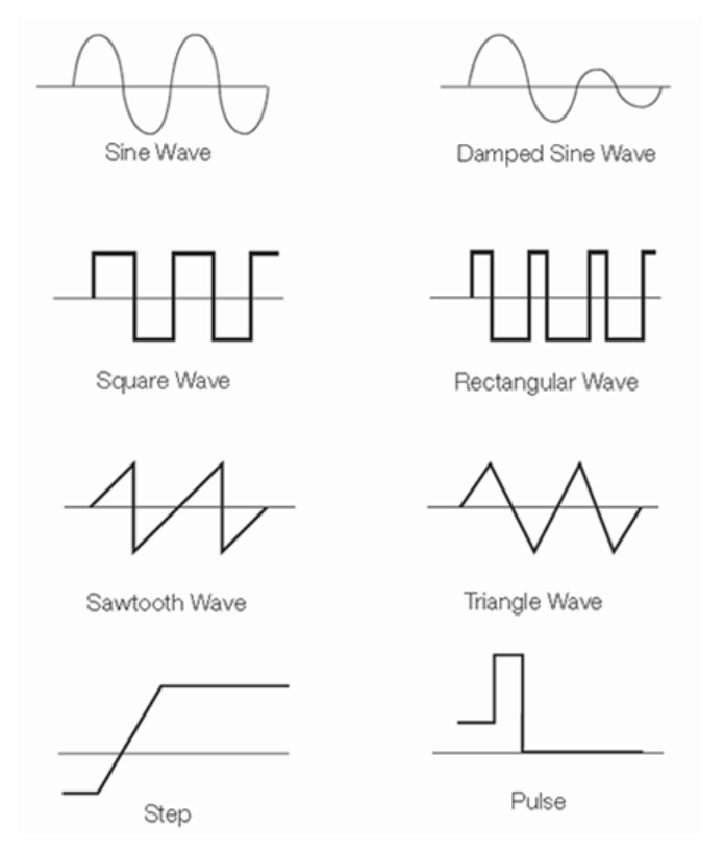
\includegraphics[width=0.45\linewidth]{img/different_pulses.eps}
    \caption{Different types of signals}
    \label{fig:signals}
\end{figure}

One can go from analog signals to digital signals by using a Analog to Digital Converter (ADC) and vice-versa by using a Digital to Analog Converter (DAC)

Digital signals have a few important properties that should be defined:

A pulse has a positive edge and a negative edge, this is when the pulse begins and ends. These edges are important for triggering, which we will see later.

A pulse has a \hl{duty cycle} which is defined by the ratio of pulse to period of the signal.

\begin{figure}[!phbt]
    \centering
    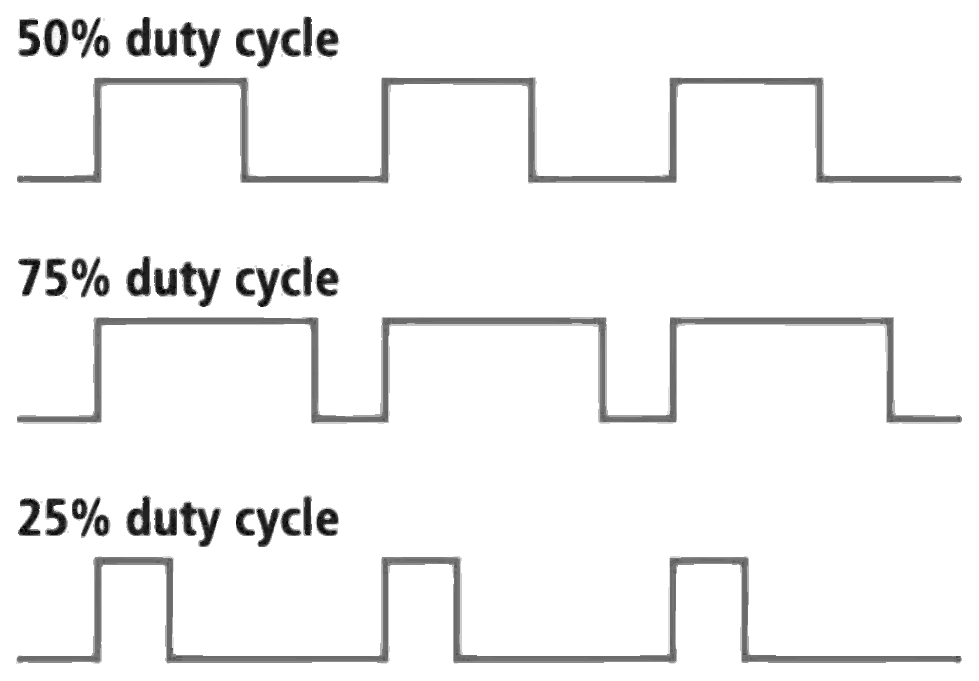
\includegraphics[width=0.45\linewidth]{img/dutycycle.eps}
    \label{fig:dutycycle}
\end{figure}

Lastly, a pulse has a point to point amplitude, $V_{pp}$ and a frequency $f$.

\subsection{Oscilloscopes}
In its most simplistic use, the Oscilloscope functions strictly as a voltage vs time measure. However, it has great versatility and deserves further explanation.

An analogy used by the Tektronix website is quite good, Oscilloscopes are similar to cameras and we must ask a few questions:
\begin{itemize}
    \item Does this picture represent what is happening?
    \item Is the picture clear or fuzzy?
    \item How many clear pictures can we take per second?
\end{itemize}

In an oscilloscope, you will have different specifications that affect your ability to get an accurate picture, let's learn about the most important ones.
\\
\
\\
Oscilloscopes have channels, the number of channels on an oscilloscope is how many signals it can read at the same time. This isn't without drawbacks as these channels often share a resource called the sampling rate.
\\
\ 
\\
Sampling rate: the sampling rate is how many times per second the voltage is measured, we will later see that this sampling rate should be at least twice the \emph{bandwidth} of the signal you're trying to measure.
\\
\ 
\\
Bandwidth: the bandwidth is the range of frequencies that your scope can reliably measure.
\\
\
\\
Every Oscilloscope will have a similar interface
\begin{figure}[!phbt]
    \centering
    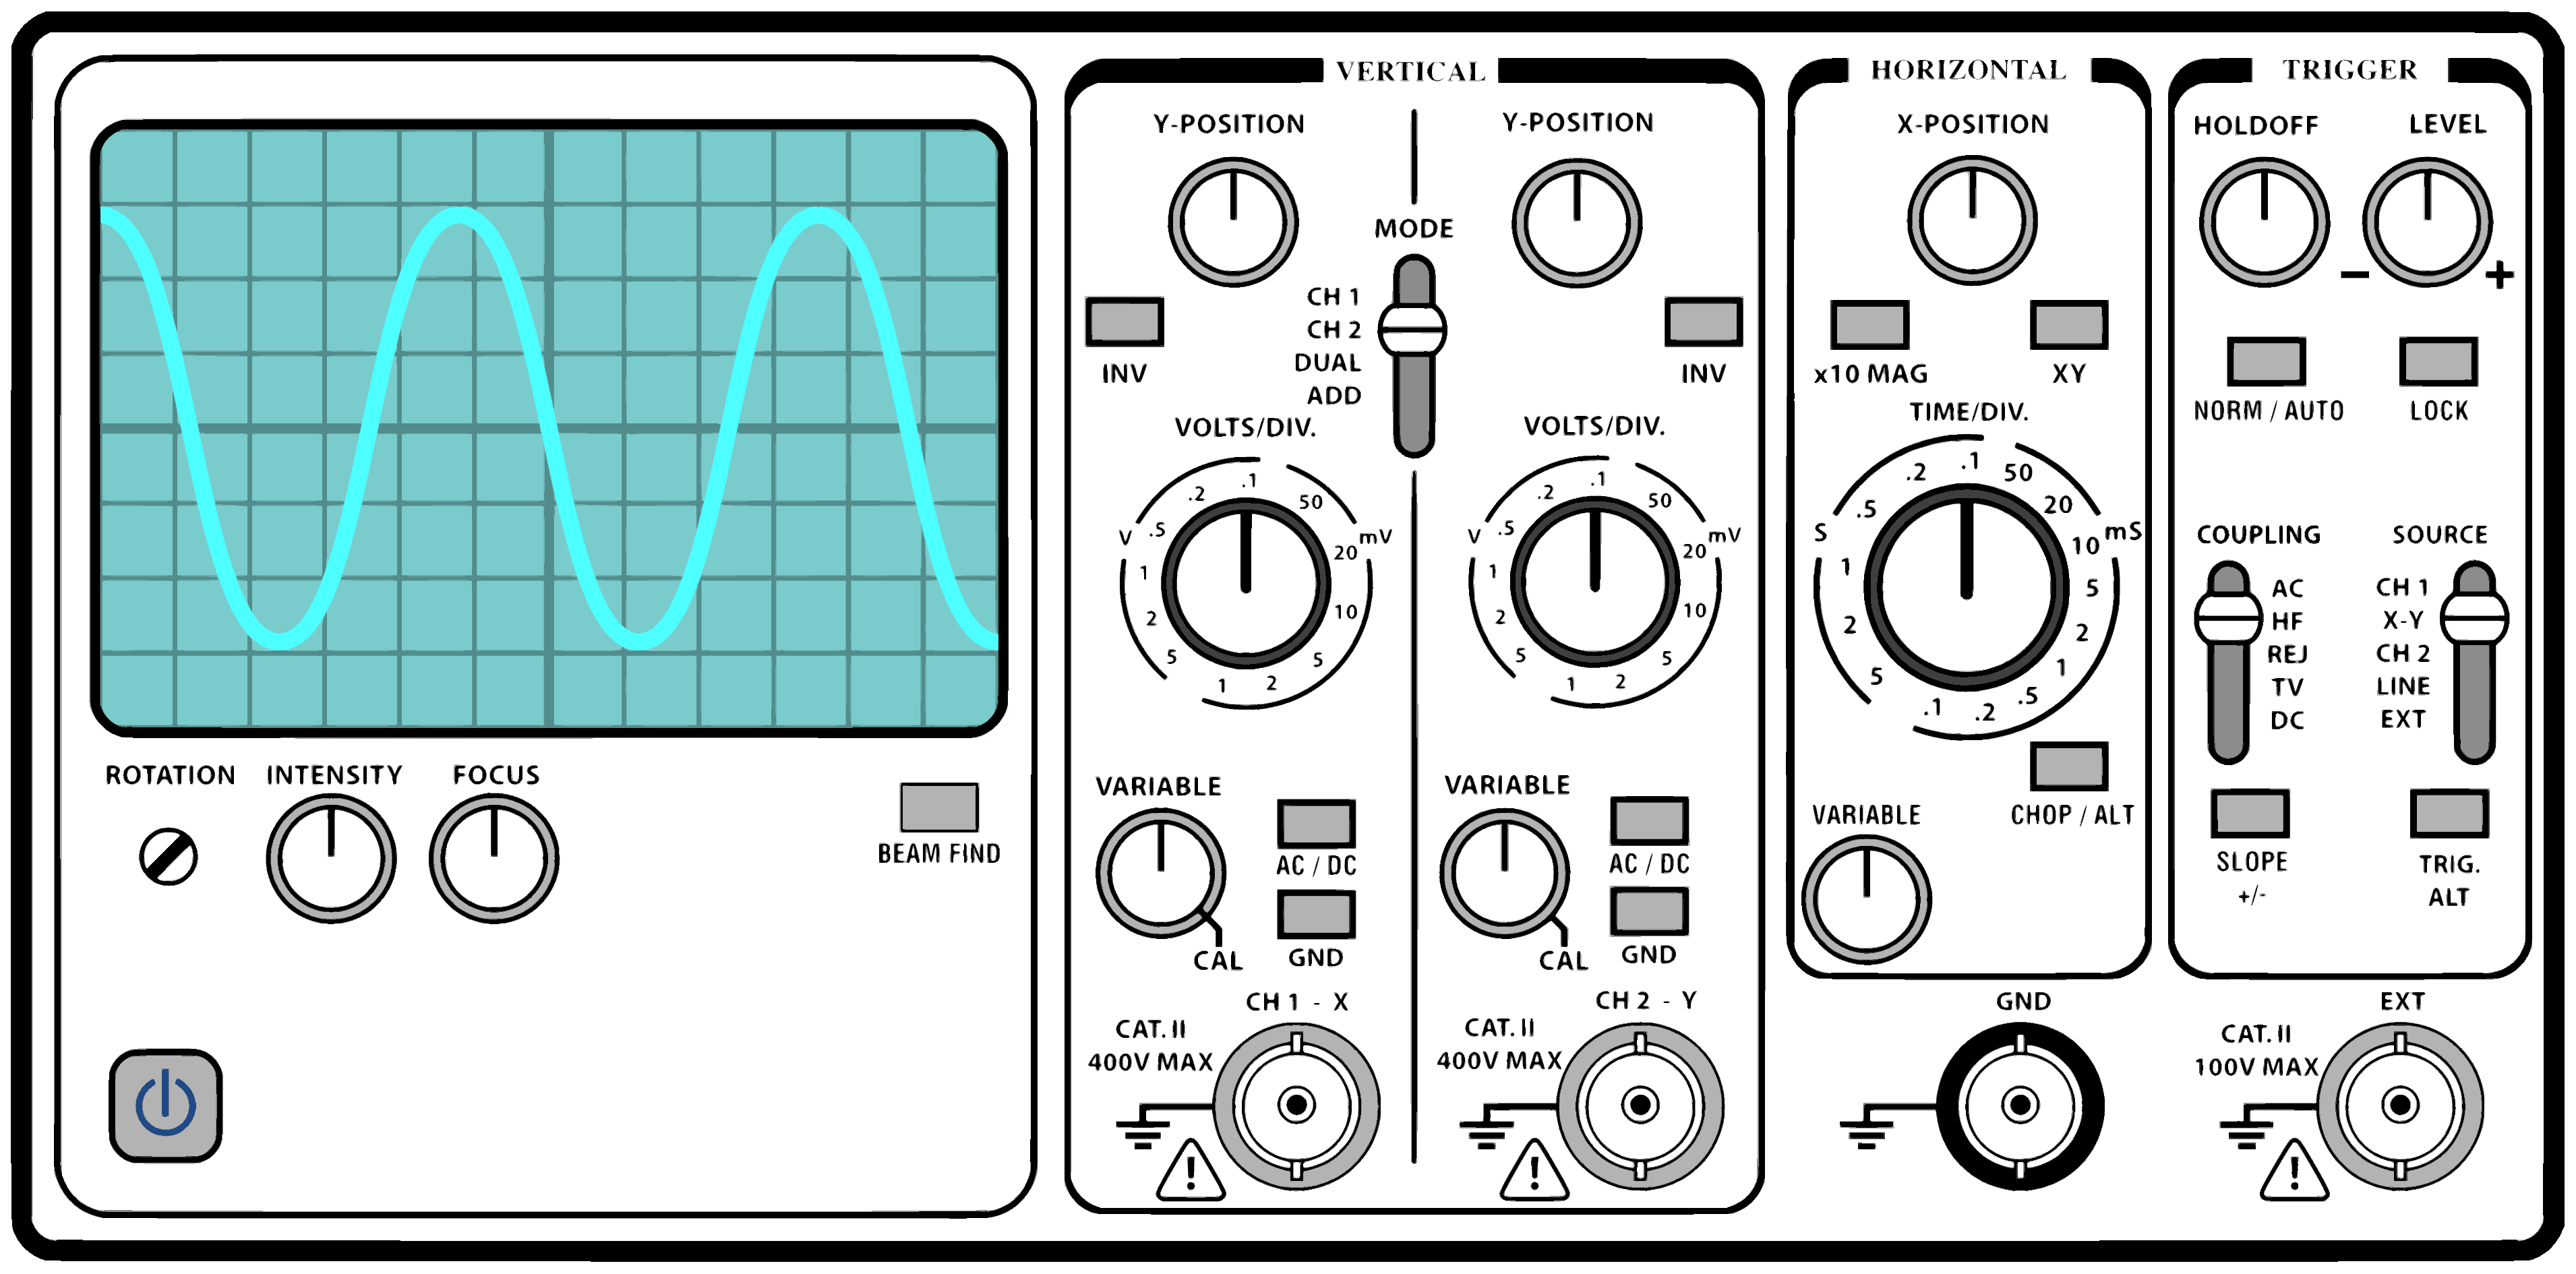
\includegraphics[width=0.85\linewidth]{img/oscilloscope.eps}
    \caption{Diagram of an Oscilloscopes interface}
    \label{fig:oscilloscope}
\end{figure}

Here we will notice the most important aspects of the oscilloscope:
\begin{itemize}
    \item X Scale Knob: This will change the scale of the x axis, you want your scale to be in the range of the frequency you're working with.
    \item Y-Scale Knob: This will change the scale of the y axis, you want your scale to be in the range of the voltage you're working with.
    \item X and Y - Position Knobs: This will allow you to change the position of the signal in the Oscilloscope, this is useful to overlap signals or shift them around.
    \item Trigger: The trigger allows you to specify when you want the Oscilloscope to start taking samples of your signal, this is the most complex aspect of the Oscilloscope and will require close attention.
\end{itemize}

One of the simplest ways to use a Trigger is to let the Oscilloscope do a voltage trigger: whenever a signal is above a certain voltage then start sampling and display it.
\\
\ 
\\

In further complexity you could set the trigger through the external input on the bottom and this will allow you to trigger the sampling process manually. 
\\
\ 
\\
There are other ways to trigger a signal such as triggering on the positive or negative edge of a pulse but, that is beyond the scope of this document.


\subsection{Nyquist Theorem and sampling}
A good resource I stumpled upon is  https://instrumentationlab.berkeley.edu/labassignments
\nocite{pentekinc}
One of the best ways to describe the Nyquist Theorem is that of a folding paper. This video does it well:

\begin{figure}[!phbt]
    \centering
    \href{https://youtu.be/pAPz5ivJaWk}{
        \scalebox{0.60}{
            \parbox{\textwidth}{
                \centering
                \textbf{A/D and D/A Sampling Theory by Pentek Inc.}\\
                \vspace{3mm}
                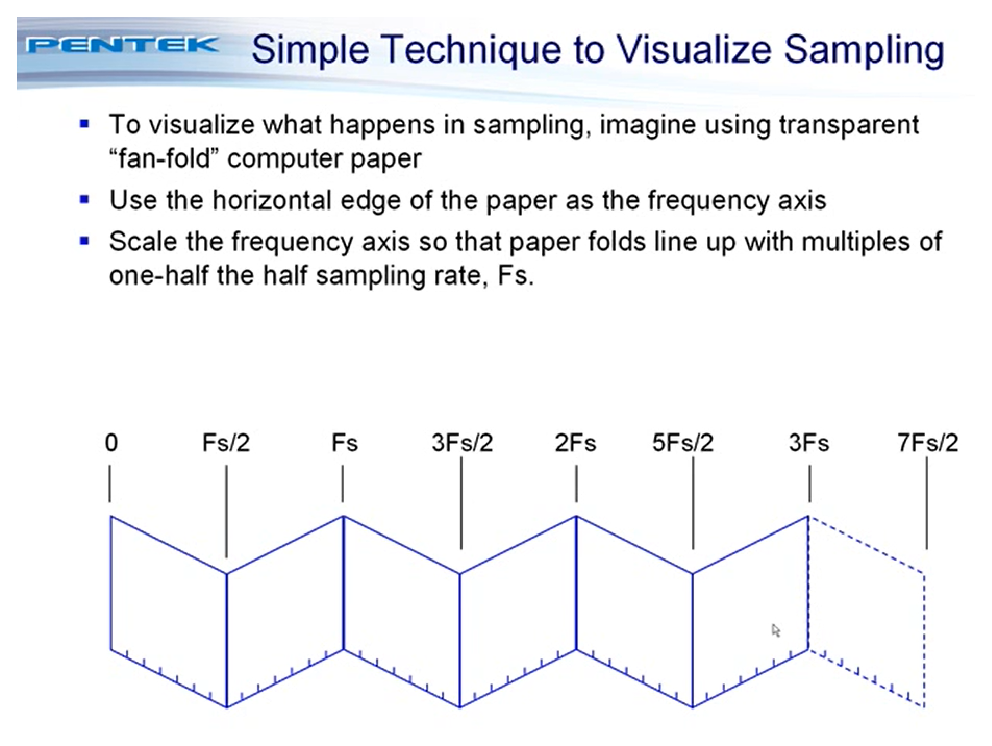
\includegraphics[width=\linewidth]{img/pentek.eps}}
        }
    }
\end{figure}
In summary, Nyquist Theorem states that the bare minimum needed to avoid aliasing (destroying of information) is \textbf{twice} the \emph{bandwidth} of the desired signal.

There are some caveats to this however, see the following examples:

\begin{figure}[!phbt]
    \centering
    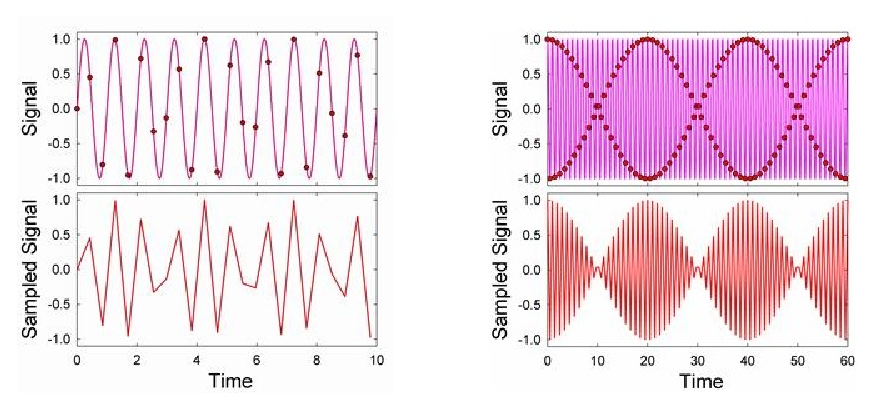
\includegraphics[width=0.65\linewidth]{img/nyquistlimit.eps}
    \caption{Two signals sampled at more than twice the Nyquist limit but, wrong sampled signals.}
    \label{fig:nyquistlimit}
\end{figure}
Both of the signals in fig. \ref{fig:nyquistlimit} were sampled at a little over the Nyquist limit, however, the sampled signal is not accurate, why?
\\
\
\\
Well if we convert the original and the sampled signals to frequency space we can see the answer.
\begin{figure}[!phbt]
    \centering
    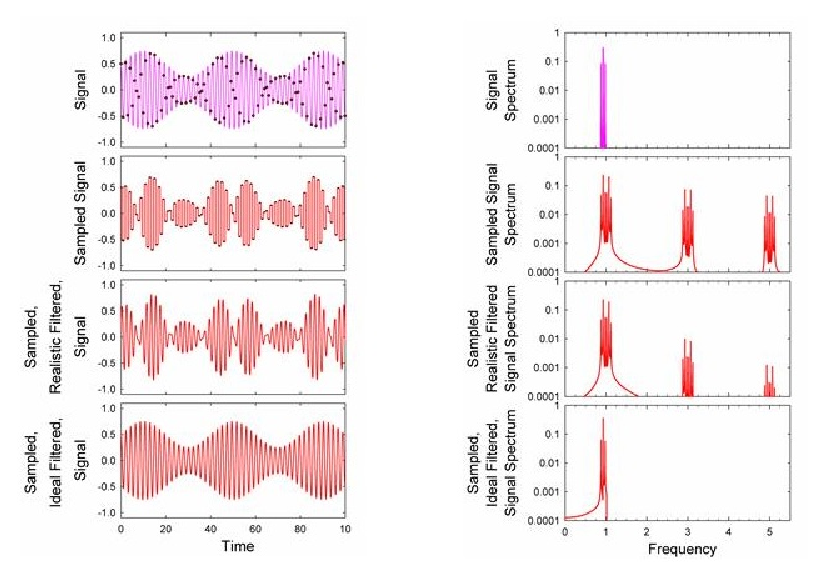
\includegraphics[width=0.75\linewidth]{img/frequencyspace.eps}
    \caption{Temporal space on the left and the corresponding frequency space on the right.}
    \label{fig:frequencyspace}
\end{figure}
\\
There appear to be additional frequencies that have to be filtered out before the original signal can be retrieved.
\\
\
\\
Signal processing is a complex and in-depth field that will require much more learning about.

\pagebreak

\subsection{Field-Programmable Gate Arrays}
Let's say you want a computer to calculate 1+1, well your input goes to the random access memory, then to the processor, through the video output and then finally you see the result of 2. However, sometimes you want to calculate things as fast as possible and so in these cases, it is inconvenient to use a processor and this long process. Instead, we will use a Field-Programmable Gate Array to compute these functions.

In order to understand how an FPGA works, we must first understand basic gates.

https://www.circuitbasics.com/what-is-digital-logic/

\begin{figure}[!phbt]
    \centering
    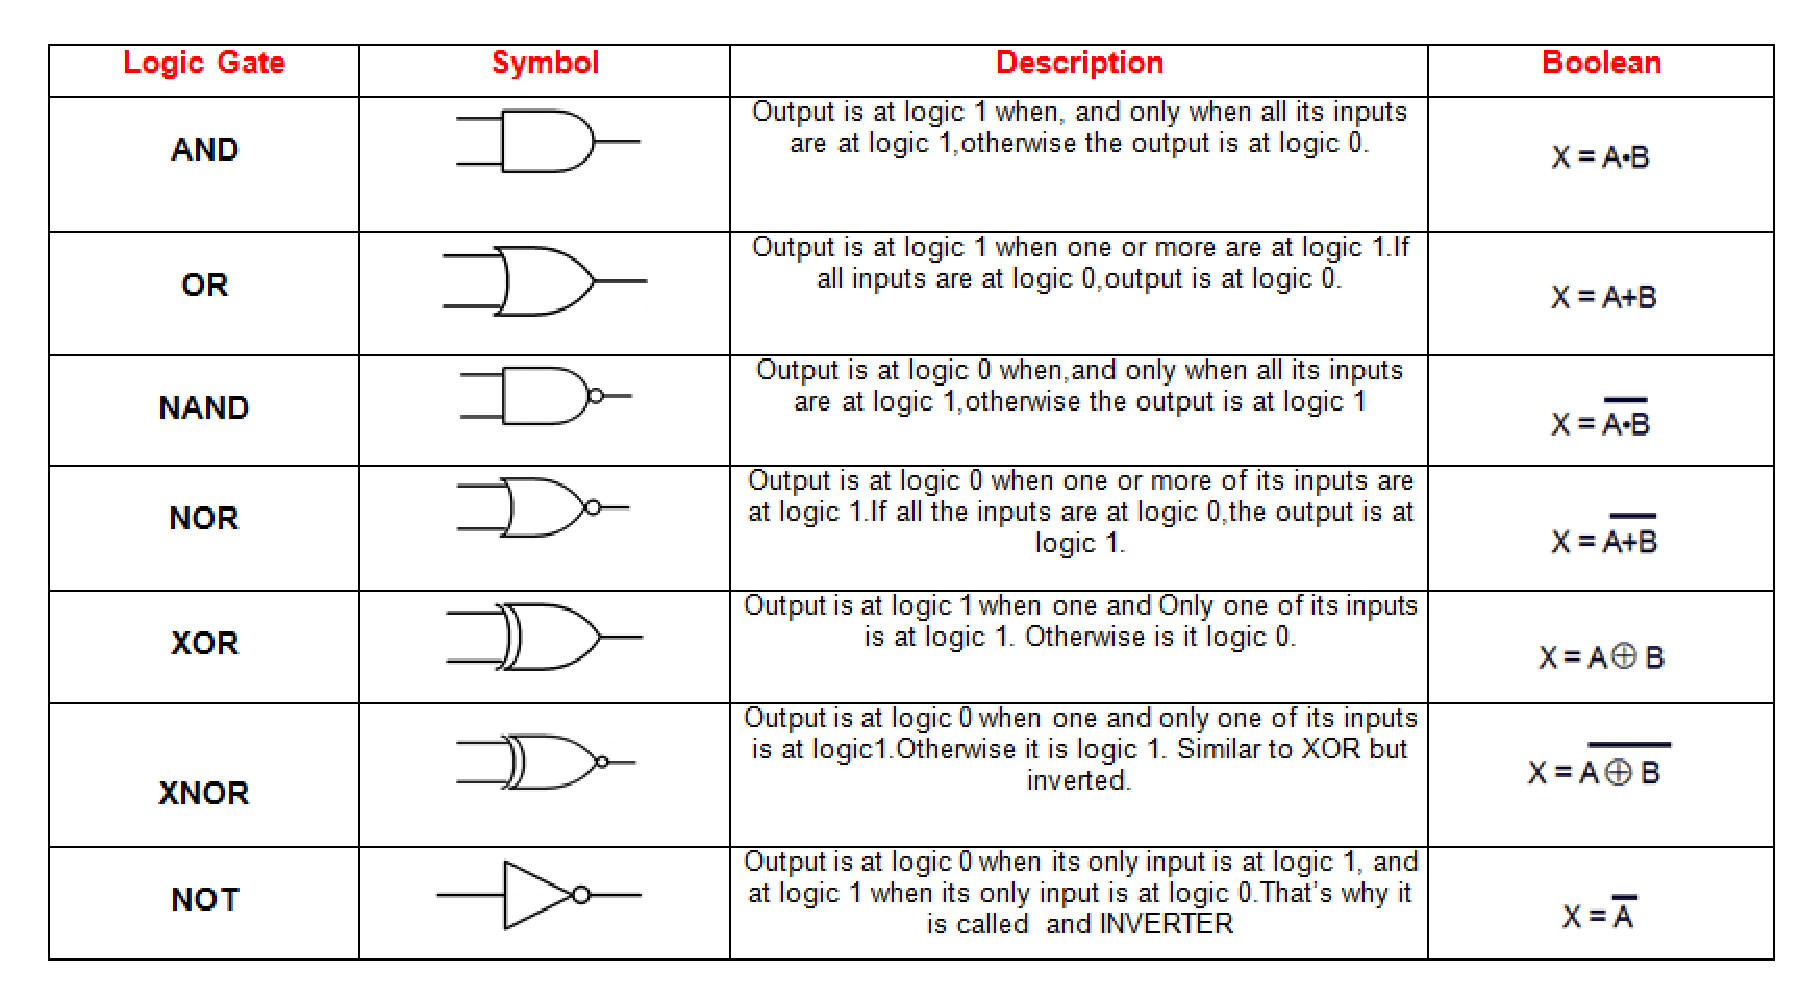
\includegraphics[width=\linewidth]{img/gates.eps}
    \caption{Gates and their outputs}
    \label{fig:gates}
\end{figure}

It is with the combination of these gates that our computers and electronics work.

There are two primary languages for HDL, Verilog and VHDL. Pick one and learn it.
\\
\
\\
For a more in-depth guide on how FPGAs work, refer to my documentation located here:


\section{Miscellaneous}

\subsection{Installing Drivers and troubleshooting}
When you plug in a USB into your computer, the computer automatically knows how to communicate with that USB and pull off any information that it needs. How does it do that?

A drivers purpose to to act as the middle man, it translates the devices functionality for the computer and without the correct driver, you will not have a properly functioning device.
\\
Here are the steps to follow when trying to install a new driver.
\begin{itemize}
    \item Step 1. Find the manufacturers website and download the driver for the device you are using (sometimes they have instructions)
    \item Step 2. Open the device manager, on windows press Win-Flag + R and type devmgmt.msc, now find the device you are trying to install drivers for.
    \item Step 2-1/2. Sometimes it is beneficial to uninstall these drivers and reinstall them if the device is not working properly.
    \item Step 3. The drivers you downloaded may have certificates that you need to install, open the file, browse through it and install any certificates if you need. (Sometimes you get unsigned certificates, google how to get around this)
    \item Step 4. On your device manager, right click your device and click install drivers and browse local files, select your driver folder or subfolders.
\end{itemize}


\subsection{Python Tutorial}
You don't really need anything to program, you can write it all in a .txt file and then compile it so the computer can interpret it. However, we usually use an IDE (Integrated Development Environment) such as Spyder, PyCharm, IDLE, or Eclipse. 
IDEs make programming easier by providing a lot of helpful resources in an easy to access manner (Like code auto-completion and error reporting)
You can use any IDE you want. I recommend PyCharm.\\

A virtual environment for all intents and purposes is just a folder which holds all the packages and modules you install under it. Conda is a package management system and environment management system, it organizes your environment and modules.
It also acts as an interpreter which is what converts your source code into stuff the computer understands.

Packages and modules are just pre-written code that you use.
Let's define a few things:
\begin{itemize}
    \item Integers: a positive or negative number
    \item Float: Decimal numbers
    \item Strings: A combination of characters
    \item Tuple: a collection of ordered and immutable (non-modifiable) objects
    \item Dictionary: A set of "key: value" pairs
    \item List: A simple array (or vector)
\end{itemize}

So, how do computers compute stuff?
Python runs code sequentially, one line after the next. Python can also only understand 1 and 0, True or False.
So we have to be careful what we tell the computer to do.

\begin{python}
# This is a comment, the computer does not read this
'''This is a multi-line
string which acts 
as a comment.'''
#This is how you assign values to variables in Python.
testInt = 5
testFloat = 5.3
testStr = "String"
testTuple = ('Hello',2,5,'Test')
testDictionary = {'A': "Apples", 'B': "Bananas"}
testList = [1,2,3]
testList2 = [[1,2,3],[4,5,6]]
#You can make a list of lists and a dictionary of dictionaries, which can be thought of as multi-dimensional arrays.
\end{python}

The next thing you should learn in Python is if else statements.
\begin{python}
if CONDITION:
    #DO SOMETHING
elif CONDITION:
    #DO SOMETHING ELSE
else:
    #DO SOMETHING ELSE^2

#This will print true since True is always true.
if True:
    print("This is always true")
\end{python}
Next thing you should learn is the two different types of loops
\begin{python}
#While Loop
while CONDITION:
    DO SOMETHING
    break #this will cause the loop to stop
    
#For loop
for VARIABLE in ITERABLE:
    #DO SOMETHING WITH VARIABLE

#Example
for k in range(50):
    print(k) #This will print the numbers 0-49 since python starts counting from 0.
while x <= 50:
    print(x)
    x = x + 1 #This will print 0-50
\end{python}
The next thing you should learn is functions
\begin{python}
def NAME(INPUT1, INPUT2,INPUT3)
    #DO STUFF WITH INPUTS
    return OUTPUT
#Functions blocks of code you can reuse whenever you want.
NAME(variable1, variable2, variable3) #Will return some OUTPUT
NAME(variable4, variable5, variable6) #Will return some other OUTPUT
\end{python}
Next thing you should learn is string formatting and the various ways you can accomplish it.
\begin{python}
#Formmatting
print('Testing\n') #Print testing and make a new line
print('Testing' + testStr) #This concatenates the two strings.
#print('Testing' + testInt) #This will not work, it will return an error
print('Testing' + str(testInt)) #This will work
print(b'01010100') #This will convert a string to bytes
print(r'Testing\nTesting\nTestinng') #This will convert the string to a raw string which will result in \n not working.
print(f'{testStr} you smell this much: {testInt}') #This will allow you to call variables in your string.
print('%s'% testStr) #Another type of formatting.
print('{} Testing {}'.format(testStr,testInt)) #Yet another way to format
\end{python}
At this point, you have a pretty decent understanding of how Python works. The best way to learn programming is by practicing and googling things until you get it to work.
To get into the advanced stuff you should learn about object-oriented programming and learn about classes. Here you are creating new object types and manipulating how they can interact with each other, for example.
\begin{python}
class NAME:
    def __init__(self,inputs): #This initializes the class and only runs once
        #DO THINGS WITH INPUTS
    def FUNCTIONMETHOD(self, optional_inputs): #This can be called as a method on the class
        #do things with optional inputs or self.methods
        
#Let's create a class called Particle
class Particle:
    def __init__(self, velocity, initial_position=(0,0),direction=(1,0)):
        self.position = initial_position
        self.direction = direction
        self.velocity = velocity
    def move(self, time):
        old_x = self.position[0]
        old_y = self.position[1]
        new_x = self.direction[0]*time
        new_y = self.direction[1]*time
        self.position = (old_x+new_x, old_y+new_y)
#We just created a particle class that has a method to move the particle
#Particle 1
Particle_1 = Particle(10, (0,0), (0,1)
#Particle 2
Particle_2 = Particle(10, (0,0), (1,0)
Particle_1.move(20)
print(Particle_1.position) #This should print the new position of particle 1
Particle_2.move(10) #This should print the new position of particle 2
\end{python}

Hopefully you can see how powerful object oriented programming can be.

Familiarizing yourself with numpy, matplotlib, scipy, sympy and making sure you are using IPython are very useful things to do.

Google everything you need and you will gather the skill of programming rather quickly.

\newpage
%--------------------------------------------------------------------------------------------------------------------------------%
\section{Experimental Tricks}
\subsection{Determine $f$ of lens}
Never take a labeled piece of optic for granted, always verify the properties of said optic.
To determine the focal length of an unknown lens, hold it up above the table until the light from the ceiling sharpens and forms an image. Then, use a ruler to measure the focal length.
\begin{figure}[!phtb]
    \centering
    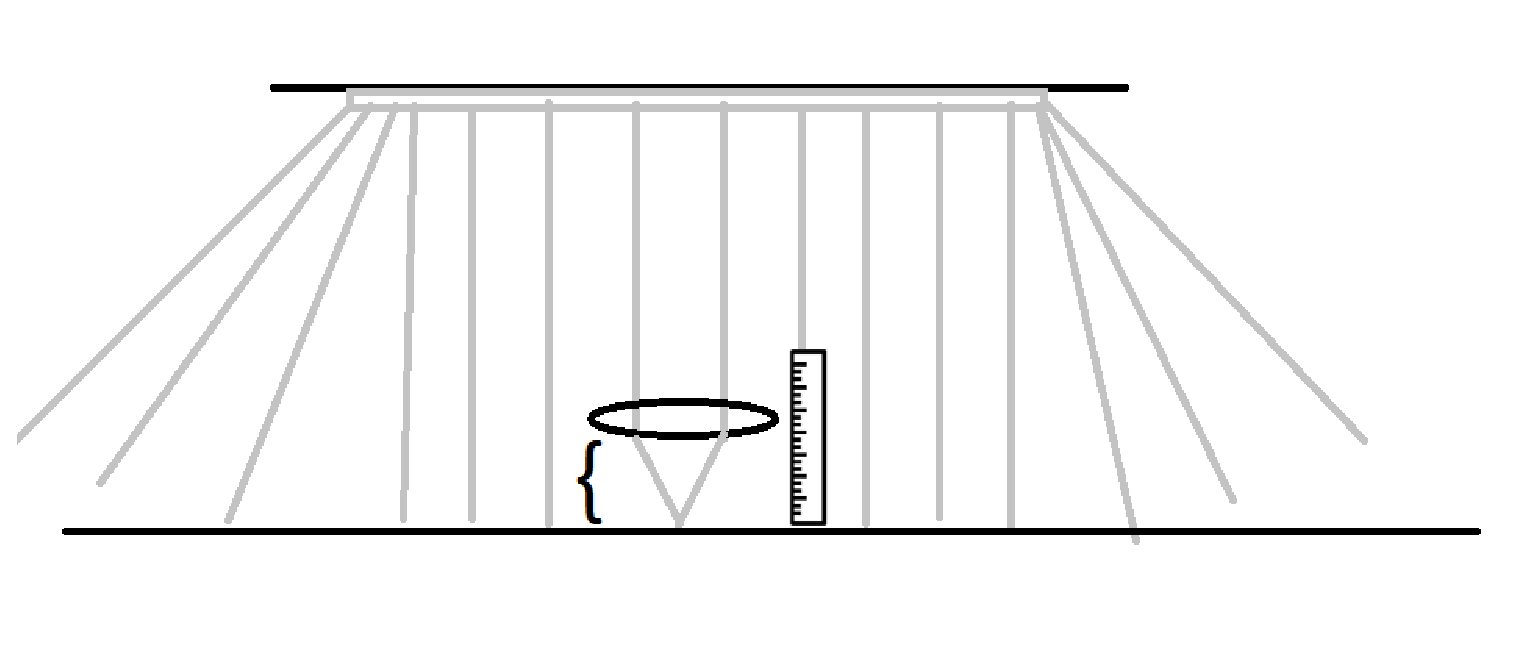
\includegraphics[width=0.5\linewidth]{img/Ceiling.eps}
    \caption{Determine focal length of unknown lens.}
    \label{fig:focallength}
\end{figure}
\subsection{Aligning a laser with two mirrors}

%--------------------------------------------------------------------------------------------------------------------------------%
\newpage

\printbibliography[heading=bibintoc]
\end{document}
